\section{Introduction}
Materials are prevalent, and have been used for thousands of years, modelled for hundreds, and manipulated for tens (making the allowance  for flamboyant language). It is therefore rather surprising that they are a relatively under-studied class of theories in certain contexts. 



Modelling a material is a game of asking rather physically simple questions: in what manner does  a substance respond under a given stimulus? What factors about the substance are important in order for useful dynamical information to be extracted? Especially information about how the substance imparts energy and momentum into surrounding materials. These concepts and associated problems are best explained by analogy.


First, suppose one wanted to construct a description of water flowing through a pipe. Given that one knows that water is constituted from ``particulate'' molecules,  one could construct a particle description. This would be built from knowledge -- or a guessed understanding -- of how water molecules interact with their neighbours and surfaces inside the pipe. With the best will and all available computing power, such a description would fail to describe almost all systems of physical interest. Instead, one moves to a coarse-grained fluids description where one attempts to describe the collective behavior of the particles on a ``large scale''.  

Secondly, suppose one wanted to construct a description of how an object, such as a table, responds to being kicked. The impact of the externally applied kick is transmitted via inter-molecular bonds within the object to release some kind of energy in the form of motion, sound, or heat.  Ones intuition has been built up to such an extent that the precise details of the inter-molecular bonds are irrelevant if one wanted to understand the large-scale response of the object to the impact. However, ones intuition well aware of the fact that if the object were made of different materials (which, on a fundamental level, means that the objects constitutive inter-molecular bonds are  different in nature), then the object could respond very differently. The amount of kicking required to move the table depends on what the table is made of (bendy, versus stiff matierials). And so, one builds a working picture of the object: it is vital to have some understanding of some of the underlying micro-physical make-up of the object when building up an understanding of the macro-physical response of the object to macro-physical impacts. 

Scalar field models of dark energy and modified gravity are prevalent in modern cosmology and it is our contention that in an important sense these are equivalent to constructing a particulate description of water, or a molecular picture of a table. We would like to offer a change in philosophy in building models.

The aims of this paper include the elucidation of the construction of non-linear material models, and  showing how ideas, schematic scenarios, and model building techniques, can be imported into the language of cosmology.

It is useful for our purposes to imagine that the theory of materials comes in two branches. The first is the theory of   \textit{continuous media}: these are supposed to be space filling substances. Relativistic realizations of such media were the subject of \cite{Bucher:1998mh, Battye:2007aa, Pearson:2014iaa}, but under the presumption that the medium was adequently described within the framework of perturbation theory (admittedly,  for the applications those studies had in mind, this was a perfectly reasonable restriction).  The second is the theory of \textit{solitons}: these are almost completely opposite to continuous media, in the sense that they are localised configurations and are highly non-linear deformations of the appropriate fields. In both descriptions of materials (i.e., continuous and localised) the idea of a map from the material manifold into space-time is heavily (and successfully) used. It appears that the important distinction between how the two types of theories are formulated is what information about the material manifold and its map is used to construct the theory.

In some sense the idea of describing a medium is similar to the idea of using multiple scalar fields to build dark energy models: the medium description is constructed with a set of three scalar fields. Except now one obtains a concrete interpretation of what the scalar fields \textit{are}. Knowing what the fields are significantly enhances physical insight, and guides the choice of  functions or parameters used to parameterize available freedom in the theory.

\begin{figure}[!t]
\begin{centering}
\tikzstyle{line} = [draw,  latex-]
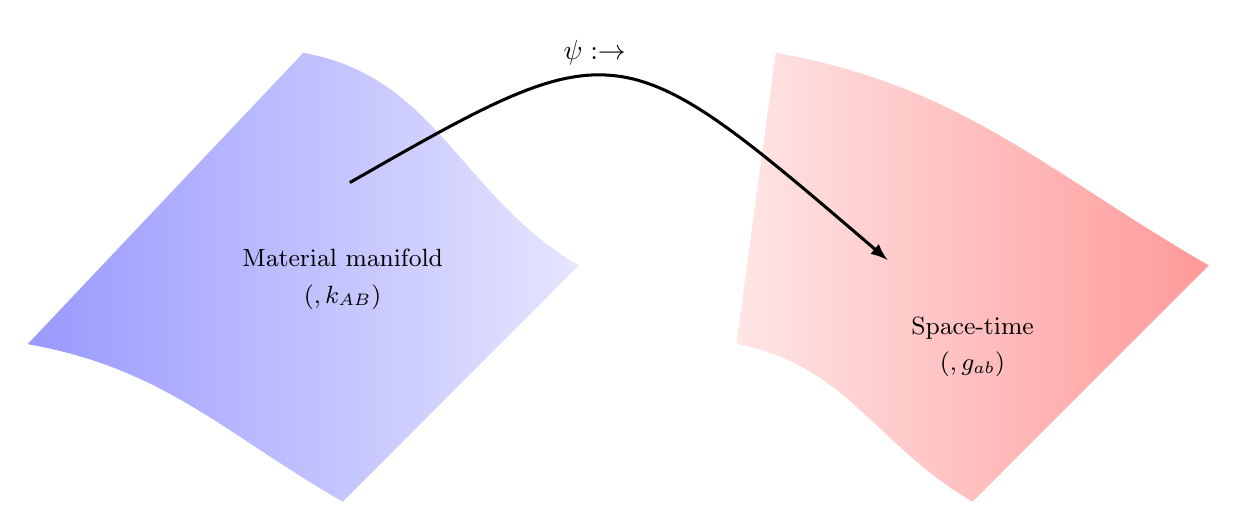
\begin{tikzpicture}
\shade[right color=blue!10,left color=blue!40] 
  (-1,0) to[out=-10,in=150] (3,-2) -- (6,1) to[out=150,in=-10] (2.5,3.7) -- cycle;
  \shade[left color=red!10,right color=red!40] 
  (8,0) to[out=-10,in=150] (11,-2) -- (14,1) to[out=150,in=-10] (8.5,3.7) -- cycle;
  % draw the map
\draw[line,black,line width=1.1pt,shorten >= 3pt,shorten <= 3pt] 
  (3,2) .. controls (6.5,4)   .. (10,1);
 
% we add some labels
\node[font=\color{black}] at (3,1.1) {{\small Material manifold}};
\node[font=\color{black}] at (3,0.6) {{\small $(\matmanif, k_{AB})$}};
\node[font=\color{black}] at (11,0.2) {{\small Space-time}};
\node[font=\color{black}] at (11,-0.25) {{\small$(\stmanif, g_{ab})$}};
\node[font=\color{black}] at (6.2,3.7) {$\psi:\stmanif \rightarrow \matmanif$}; 
\end{tikzpicture}
\caption{Schematic depiction of the  map $\psi$ that associates a point in the material space $\matmanif$ with a point in space-time $\stmanif$. We have also shown which metric is associated with which manifold (and the associated labelling of the indices).}\label{fig:shem_map}
\end{centering}
\end{figure}

\begin{itemize}
\item In Bucher and Spergel, \cite{Bucher:1998mh}, the linearized theory is constructed in detail.
\item See Carter and Quintana \cite{Carter21111972, Carter:1977qf}, Karlovini \cite{Karlovini:2002fc, Karlovini:2003xi, Karlovini:2004gq, Karlovini:2007ut} and \cite{Beig:2002pk, Frauendiener:2007yx, Brito:2009jj, Pourtsidou:2013nha}; \cite{Battye:2005ik}
\cite{Balthazar:2014oza} and \cite{Dubovsky:2011sj}
\item Elasticity and ``hyper -elasticity'' have been further developed in \cite{Carter:1982xm}, \cite{Carter:2006cw}
\item The pull-back idea is very similar to the restoration of non-linear diffeomorphism invariance utilised by massive gravity theories \cite{deRham:2014zqa}.
\item See effective field theory of perfect fluids, \cite{Ballesteros:2012kv}
\item Note that \cite{Karlovini:2002fc} take the tensor $k_{AB}$ to be fixed on the material space.
\item see \cite{Bel:1996pb} \cite{Polak:2007dm}
\item Solids in inflation context \cite{Gruzinov:2004ty, Endlich:2012pz, Bartolo:2014xfa}
\item see \cite{Skovran:2014dka} for exact analytic solutions for perturbed single-component cosmology 
\item \cite{Frauendiener:2007yx}, \cite{Kijowski:1994eq}
\item Carter and elastic theory for neutron stars \cite{Carter:2005gg}
\item Relativistic hydrodynamics lecture notes \cite{Gourgoulhon:2006bn}
\end{itemize}

\subsection{Deformation theory and cosmology}
The current state of affairs in cosmology is that the Universe is accelerating in its expansion. A huge business has boomed with the expressed intention of explaining this observation; this has yielded a huge literature of both phenomenologically and theoretically motivated modifications to gravity. The summary is that the prediction obtained from General Relativity (GR) for how the Universe should look doesn't match up with observations of how the Universe does look (unless, for example, some form of exotic matter is included). 

One popular way of understanding how to tackle this mis-match is to write the gravitational field equations that actually describes the Universe as
\bea
G_{ab} = 8 \pi G \left(T_{ab} + U_{ab}\right).
\eea
Here, $G_{ab} = R_{ab} - \tfrac{1}{2}Rg_{ab}$ is Einstein's tensor, and $T_{ab}$ is the energy-momentum tensor of all \textit{known} matter sources (such as radiation, baryonic, and dark matter).
The tensor $U_{ab}$ is the dark energy-momentum tensor, and contains all the deviations or deformations (to begin using the terminology we aim to develop) of the field equations which describe the actual Universe away from the GR (+ standard matter content) predictions. 

The modern cosmology community is busy with developing candidate theories which could provide the components of the tensor $U_{ab}$. The focus is also on working out the observational consequences of their given form of the tensor by using observational probes such as the distances to supernovae, the Cosmic Microwave Background radiation, and the effects of the evolution of gravitational perturbations on the propagation of photons.  

These candidate theories usually fall into the class of ``dark energy'' or ``modified gravity'', and are generally constructed in order to satisfy mathematical principles. Whilst this is an entirely sensible philosophy (the principle of building models whilst asking for symmetries to hold has served theoretical physics very well), we  would like to suggest a different approach, or at least, a different philosophy for attacking the problem. Explaining this approach, and showing how it can be used, is the subject of this paper.

In the theory of deformations (in particular, we have in mind   theories of relativistic elasticity) one imagines two states of a material. The first state is a relaxed configuration, and the second is a strained configuration. The deformation which was imparted on the material to take it from being relaxed to being strained isn't necessarily small (if it was small, one would  speak about linear elasticity theory). The theory of deformations prescribes a tool-kit for writing down terms in the field equations which are allowed, given classes or categories of deformation. For example, if the deformation is performed ``on'' some perfect fluid or perfect solid, then it is known that the quantities $U_{ab}$ takes on the form
\bea
\qsuprm{U}{\{fluid\}}_{ab} = \rho u_au_b + P\gamma_{ab},\qquad \qsuprm{U}{\{solid\}}_{ab} = \rho u_au_b + P_{ab}.
\eea
The energy-momentum tensors written above \textit{become} those for a fluid or solid when some extra theoretical structure is used. Namely, an \textit{equation of state}. For readers who are used to the literature in modern cosmology, this phrase is often used to describe the link between the dark energy pressure $P$ and density $\rho$, via an equation of the form $P(t) = w(t) \rho(t)$. In the context of material models, an equation of state is the Lagrangian density.

When one constructs ``conventional'' models of dark energy or modified gravity, one has a some freedom to choose various types of quantities: these are, e.g., functional forms of the potential, or the kinetic terms which appear in the Lagrangian density. This may seem like an obvious point, but the choice of a restriction on a theory can have implications for (a) its applicability, and (b) its physical naturalness/interpretation. This is a particularly pertinent point, and so therefore we want to take inspiration from the extremely well developed field of the \textit{mechanics of solids} and use that as a model building guide.


\subsection{Fluids and solids}
The distinction between a \textit{fluid} and a \textit{solid} isn't one of the best explained concepts in the literature. Fluids are commonly used as a description for the ``source term'' in a gravitational theory, since they are both mathematically simple and physically intuitive. But fluids are only a sub-class of a more general description for ``content''. To perhaps use a  more physically transparent terminology: for materials. A more general  description of material is that of a solid; obviously, we won't go so far as to say \textit{the}  general material description. Below we will outline some of the salient pieces to the construction of a material model: full explanations are given in the rest of this paper.

In the descriptions of both solids and fluids  one has a notion of a \textit{material metric} $k_{AB}$ on a \textit{material space}, whose determinant is related to the particle number density, $n = \sqrt{\det k_{AB}}$. A convenient decomposition of this metric is $k_{AB} = n^{2/3}\eta_{AB}$. With this decomposition of   $k_{AB}$, the conformal metric $\eta_{AB}$ is uni-modular, i.e., it has unit determinant. Note that all indices are of ``capital latin'' type: this indicates that they correspond to quantities defined on the material manifold. Such quantities can be ``pulled-back'' to the space-time manifold. For example, the components of the uni-modular tensor in the space-time manifold are constructed from the set of three scalars $\phi^A$  and $k_{AB}$ via
\bea
\eta_{ab} = n^{-2/3}k_{AB}\partial_a\phi^A\partial_b\phi^B.
\eea
The $\phi^A$ are the coordinates on the material manifold: physically they specify the locations of the particles.

The action for the material is constructed by integrating the Lagrangian density whose arguments are all possible scalar quantities formed from the available structures in space-time which are the pulled-back counterparts of structures on the material manifold. Schematically put, the material Lagrangian can be written as $\ld = \ld({k^a}_b)$, although this has not yet made manifest the scalar arguments.
The action for both a fluid and a solid is of the general form 
\bea
\label{eq:intro-solid-action}
S = \int \dd^4x\, \sqrt{-g}\, \ld\left(n, \left[ \gbm{\eta}\right],\left[\gbm{\eta}^2\right]\right).
\eea
The square-braces in (\ref{eq:intro-solid-action}) denote traces of the mixed components of the uni-modular tensor, ${\eta^a}_b = \gamma^{ac}\eta_{cb}$. 

It is useful to split up the Lagrangian density   as $\ld = n \epsilon$, where $\epsilon$ is the energy per particle and $n$ retains its interpretation as the particle number density. In the  cases of   fluids or solids, $\epsilon$ is a function with the following dependencies:
\bea
\qsubrm{\epsilon}{fluid} = \qsubrm{\epsilon}{fluid}(n),\qquad \qsubrm{\epsilon}{solid} = \qsubrm{\epsilon}{solid}(n, {\eta^a}_b).
\eea
This makes the distinction between solids and fluids explicit: it is the dependence of the energy per particle on the uni-modular tensor ${\eta^a}_b$ which makes the description that of a solid rather than of a fluid. Later on we will see that the physical consequence of this dependence is that the substance is able to support anisotropic stress (whereas fluids can't): this manifests as \textit{rigidity}. It is worth noting that a fluid is a highly symmetric solid, and a pressureless fluid has $\qsubrm{\epsilon}{fluid}(n) = \overline{\epsilon}_0$, a constant.

Solids and fluids are only two examples of a more general category of ``material models''. In \fref{fig:shem_roadmap} we name a few other classes of materials: such as viscous and plastic ones. We have also pointed out how some of the examples are related, and the current applications of some of the types.


\tikzstyle{block} = [fill=red!20, draw,rectangle,  text centered, rounded corners, minimum height=2em]
\tikzstyle{block2} = [fill=blue!20,draw,rectangle,  text centered, rounded corners, minimum height=2.5em]
\tikzstyle{block3} = [fill=green!20,draw,rectangle,  text centered, rounded corners, minimum height=2em]
\tikzstyle{block4} = [fill=yellow!5,draw,rectangle,   dotted, text centered, rounded corners, minimum height=2em]

\tikzstyle{line} = [draw,  -latex,   thick]
\tikzstyle{line2} = [draw,  latex-,   thick]
\tikzstyle{cloud} = [ minimum height=2em]

\begin{figure}[!t]
\begin{centering}
\begin{tikzpicture}[node distance = 2cm, auto]
    % Place nodes
    \node [block2] (materialmodels) {{\bf Material models}};
    \node [block3, right of=materialmodels, node distance=5cm] (imperfect) {Viscous};
%    \node [block3, left of=materialmodels, node distance=7cm] (kv) {Visco-elastic solid};
    \node [block3, below right = 1.5cm of materialmodels, node distance=2cm] (solid) {Solid};		
    \node [block3, above left = 1.5cm of materialmodels, node distance=2.5cm] (mixtures) {Mixture};
    \node [block3, above right = 1.5cm of materialmodels, node distance=5cm] (plastic) {Plastic};    
    \node [block3, below left = 1.5cm of materialmodels, node distance=5cm] (fluids) {Fluid};
    \node [block4, below left = 0.5cm of solid, node distance=5cm] (cosmology) {\small Cosmology};
    \node [block4, below right = 0.5cm of solid, node distance=4cm] (nonlinear) {\small Compact objects};
        \node [block, above right = 1.25cm of mixtures, node distance=2cm] (solidscalar) {\small Solid+scalar};
        \node [block, right of=solidscalar, node distance=4cm] (fluidscalar) {\small Fluid+scalar};        
    % Draw edges
    \draw [line] (materialmodels) -- node{\scriptsize perfect}(solid);
    \draw [line] (materialmodels) -- node{\scriptsize example}(fluids);
    \draw [line] (materialmodels) -- node{\scriptsize imperfect}(imperfect);
    \draw [line] (materialmodels) -- node{\scriptsize extra}(mixtures);    
    \draw [line] (materialmodels) -- node{\scriptsize extra}(plastic);        
    \draw [line] (solid) -- node{\scriptsize zero rigidity}(fluids);     
    \draw [line] (solid) -- node{\scriptsize linear}(cosmology);        
    \draw [line] (solid) -- node{\scriptsize non-linear}(nonlinear);           
%    \draw [line] (kv) --  node{\scriptsize Kelvin-Voigt}(cosmology);             
    \draw [line] (mixtures) -- node{\scriptsize hyper-elastic}(solidscalar);             
    \draw [line] (solidscalar) -- node{\scriptsize sub-case}(fluidscalar);         
%    \draw [line] (kv) --  (cosmology);                                
\end{tikzpicture}
\caption{Road-map containing some of the simplest material models. This picture coarsely shows how some of the common classes of materials are related. For example, we see that a fluid is a perfect solid with zero rigidity. We have also shown that the linear theory of solids has been applied to cosmology, and the non-linear theory to compact objects (such as neutron stars).}\label{fig:shem_roadmap}
\end{centering}
\end{figure}
 

{\renewcommand{\arraystretch}{1.4}
\begin{table}%[b] 
%\begin{andptabular}{X[4c]X[4c] }%
\begin{center}
\begin{tabular}{||c |  c ||}
%{Summary  of    commonly used symbols}
\hline
\textbf{Symbol} & \textbf{Meaning} \\
\hline
$\lied{X}$ & Lie derivative operator along the vector $X^{\mu}$\\\hline
$\left(\stmanif, g_{ab}\right)$ & Space-time manifold and metric\\\hline
$\left(\matmanif, k_{ab}\right)$ & Material manifold and metric \\\hline
$u_a$ & Time-like unit-vector; $u^au_a = -1$\\\hline
$\gamma_{ab} = g_{ab} + u_au_b$ & Orthogonal projector; $u^a\gamma_{ab}=0$\\\hline
$n$ & Particle number density; $n^2 = \det k_{AB} $\\\hline
${\eta^a}_b = n^{-2/3}{k^a}_b$ & Uni-modular tensor\\\hline
$\epsilon$ & Equation of state
\\\hline
\end{tabular}\caption{Summary of commonly used symbols}\label{tab:common}
\end{center}
\end{table}
}

Another  concept which is used is that of a \textit{perfect fluid}. This is supposed to be a substance whose energy-momentum tensor can be put into the form $T_{ab} = \rho u_au_b + P\gamma_{ab}$,
in which $\rho$ and $P$ are the  fluid's energy density and pressure respectively, $u^a$ is the velocity of the fluid and $\gamma_{ab} = g_{ab} + u_au_b$ is the orthogonal projection operator. If the energy-momentum tensor for a \textit{fluid} is not of this form (for example, if there is anisotropic stress or heat flux) then the \textit{fluid} is said to be   \textit{imperfect}. We are deliberately being careful about only using the term \textit{fluid}: a solid can be categorised in a similar sense, but a perfect solid manifestly has an anisotropic part to the energy-momentum tensor (this  distinguishes a solid from a fluid).


In some sense the  goal of this review is to obtain an understanding of the theory of a relativistic solid: useful geometric structures on the manifold of particle locations, the action, and energy-momentum tensor. It is rather involved, but is worthwhile since expressions and formulae obtain physical meaning.

\subsection{Conventions}
We use   lower-case latin letters, $a,b,c,\ldots$ to denote space-time indices, and upper-case latin letters, $A, B, C, \ldots$ to denote  indices on the material manifold. The space-time metric is decomposed as
\bea
\label{decomp_g-u-h}
g_{ab} = \gamma_{ab} - u_au_b,
\eea
in which $u_a$ and $\gamma_{ab}$ are the 4-velocity and spatial metric, satisfying
\bea
u^au_a = -1,\qquad u^a \gamma_{ab}=0.
\eea
We use the orthogonally projected derivative
\bea
\label{eq:orth-proj-deri-defn}
\overline{\nabla}_a{A^{b\cdots}}_{c\cdots} = {\gamma^{d}}_a{\gamma^b}_e\cdots {\gamma^f}_c\cdots\nabla_d{A^{e\cdots}}_{f\cdots}
\eea
and the expansion (extrinsic curvature) tensor
\bea
\Theta_{ab} =\overline{\nabla}_{(a}u_{b)}.
\eea
It immediately follows that $\overline{\nabla}_a$ is the connection compatible with $\gamma_{ab}$, since
\bea
\label{eq:sec:overlinenabh=0}
\overline{\nabla}_a \gamma_{cd} =0.
\eea
We will use angular braces to denote the symmetric, trace-free part of a tensor:
\bea
\label{ttls-defin}
A_{\langle ab\rangle} = A_{(ab)} - \tfrac{1}{3}{A^c}_c \gamma_{ab}.
\eea
%    \subsubsection{First, second, and third fundamental tensors}
%    Here we briefly review some of Carter's technology \cite{Battye:1995hv, Carter:2000wv, Carter:2011ab} for dealing with branes and imbeddings. 
%    
%    The idea is that writing ${x^{\mu}}_{,i} = \partial x^{\mu}/\partial \sigma^i$, with $\sigma^i$ the worldsheet coordinates, induces a metric on the world-sheet, $\overline{g}_{ij} = g_{\mu\nu}{x^{\mu}}_{,i}{x^{\nu}}_{,j}$. Instead of working with this quantity (which is written in terms of worldsheet coordinates), it is much more convenient to work with $\overline{g}^{\mu\nu} = \overline{g}^{ij}{x^{\mu}}_{,i}{x^{\nu}}_{,j}$. This invites decomposition of  the space-time metric according to
%    \bea
%    \label{eq:sec:decomp_brane_g}
%    g_{\mu\nu} = \overline{g}_{\mu\nu} + \perp_{\mu\nu}.
%    \eea
%    Here $\overline{g}_{\mu\nu}$ is the world-sheet tangential metric: it is the first fundamental form. Also, $\perp_{\mu\nu}$ is orthogonal to the world-sheet. These satisfy
%    \bea
%    \overline{g}_{\mu\nu} {\perp^{\mu}}_{\alpha}=0,\qquad \overline{g}_{\beta\nu}\overline{g}^{\alpha\nu} = {\overline{g}^{\alpha}}_{\beta}.
%    \eea
%    The  space-time covariant derivative projected into the world-sheet is
%    \bea
%    \overline{\nabla}_{\mu} = {\overline{g}^{\alpha}}_{\mu}\nabla_{\alpha}.
%    \eea
%    The second fundamental tensor is defined via
%    \bea
%    {K_{\mu\nu}}^{\rho} = {\overline{g}^{\sigma}}_{\nu}\overline{\nabla}_{\mu}{\overline{g}^{\rho}}_{\sigma}.
%    \eea
%    The first fundamental tensor determines the tangential derivative of the world-sheet metric via
%    \bea
%    \label{eq:sec;Kmuab-defn-1}
%    \overline{\nabla}_{\mu}\overline{g}_{\alpha\beta} = 2 K_{\mu(\alpha\beta)}.
%    \eea
%    The second fundamental tensor satisfies
%    \bea
%    {\perp^{\mu}}_{\alpha}{K_{\mu\nu}}^{\lambda}=0,\qquad {\overline{g}_{\lambda}}^{\sigma}{K_{\mu\nu}}^{\lambda}=0.
%    \eea
%    It is convenient to introduce the extrinsic curvature vector as the trace of the first fundamental tensor,
%    \bea
%    K^{\mu} \defn {K^{\alpha}}_{\alpha}{}^{\mu},
%    \eea
%    which satisfies
%    \bea
%    {\overline{g}^{\mu}}_{\nu}K^{\nu}=0.
%    \eea
%    
%    The third fundamental tensor is 
%    \bea
%    {\Xi_{\lambda\mu\nu}}^{\rho} \defn {\overline{g}^{\sigma}}_{\mu}{\overline{g}^{\tau}}_{\nu}{\perp^{\rho}}_{\alpha}\overline{\nabla}_{\lambda}{K_{\sigma\tau}}^{\alpha}.
%    \eea
%    
%    
%    The more common decomposition of (\ref{eq:sec:decomp_brane_g}) comes in the 3+1 form, via the identifications
%    \bea
%    \overline{g}_{\mu\nu} = \gamma_{\mu\nu},\qquad \perp_{\mu\nu} = u_{\mu}u_{\nu}.
%    \eea
%    \bea
%    \nabla_{\mu}\gamma_{\alpha\beta}  =2K_{\mu(\alpha}u_{\beta)}.
%    \eea
%    \bea
%    K_{\mu\alpha\beta} = K_{\mu(\alpha}u_{\beta)}
%    \eea
%    It follows that (\ref{eq:sec;Kmuab-defn-1}) evaluates to
%    \bea
%    \overline{\nabla}_{\mu}\gamma_{\alpha\beta}.
%    \eea
%    
%    
%    
%    
%    


\section{Describing non-linear materials}
In this section we will take some time to build a description of a medium. We will introduce the notion of a material manifold, and geometric structures on the material manifold: coordinates, metric, connection, and volume form. There will be an important step where we relate structures in the material manifold to structures in space-time. We will want to obtain fields and energies in space-time due to structures in the material manifold. There will be some instances where we ``mix'' material space and space-time indices; this is   unavoidable in the course of exposing some interesting part of the formalism. That said, all final results (equations of motion etc) will be expressed solely in terms of space-time indicies.
\subsection{The material manifold,  particle number density, and map}
\label{sec:mpnd}
One imagines that there is a continuous distribution of particles in the space-time manifold, $\stmanif$. These particles carve out world-lines. In order to specify the location of the particle, one can attach three coordinates to a given world-line. The set of these three-coordinates forms the \textit{material manifold}, which we denote by $\matmanif$. We  assume that the 3D material manifold $\matmanif$   is endowed with a particle density form, denoted by $n_{ABC} = n_{[ABC]}$.  The integral of $n_{ABC}$ over some region in $\matmanif$ tells us about the number of particles of the medium that reside in that region. We will also assume that there is an associated metric on the material manifold, which we call $k_{AB}$, but we will discuss it   later on. 

The points of $\matmanif$ are  particles of the medium, and they do not move: the dynamics in space-time comes from the maps from the material manifold to space-time, not the motion of the particles in material space.  This is enforced by a condition we explain below. 

 Now suppose that  $\stmanif'$ is the submanifold of the full space-time manifold $\stmanif$ that the material passes through. Then invoke a map $\psi$ which takes a location in space-time and points at a location in the material manifold;
\bea
\label{eq:sec:mapdefn}
\psi : \stmanif'\longrightarrow \matmanif.
\eea
For all points p in $\matmanif' = \psi(\stmanif')$, the inverse map at that point, $\psi^{-1}({\rm p})$, is a single time-like curve in $\stmanif'$: these are the flow-lines of the particles. This construction is the analogue of allowing a scalar field, $\phi$ say, to pervade the Universe: for a real scalar field $\phi$, rather than (\ref{eq:sec:mapdefn}) one has $\phi : \stmanif\rightarrow \mathbb{R}$.

Let $\phi^A$ be   coordinates in material space. Then their gradients with respect to the space-time coordinates $x^a$ can be computed
\bea
\label{eq:sec:config_gradient}
{\psi^A}_a \defn \pd{\phi^A}{x^a} = {\phi^A}_{,a} = \partial_a\phi^A;
\eea
in which we have given the definition of the ${\psi^A}_a$ and a list of useful notational alternatives.
The ${\psi^A}_a$ are   the components of the configuration gradient. These would be the components of the Jacobian associated with a coordinate transformation if the dimension of the material manifold were to be the same as the dimension of the space-time manifold. 

The enforcement of  the material coordinates being static with respect to changes in coordinate time, or in orther words that a given world-line corresponds to a given particle, is that the time-like projection of the configuration gradients must vanish
\bea
\label{eq:sec:ortho-condition}
u^a{\psi^A}_a =0.
\eea
This is equivalent to setting the Lie derivative of the $\phi^A$ in the time-like direction to zero:
\bea
\lied{u}\phi^A=0.
\eea
It can be useful to imagine that the whole world-line of a particle in space-time is associated with one point on $\matmanif$, in which case the value of the coordinate on $\matmanif$ cannot be dependent upon the ``time'' coordinate. Thus, (\ref{eq:sec:ortho-condition}) must hold.
If the condition (\ref{eq:sec:ortho-condition}) is relaxed one ends up describing ``hyper-elastic'', rather than ``elastic'' theories, and bears resemblance to a theory which mixes a scalar with a solid. That case has been pointed out by Carter [], and will not be further explored in this review.

One can conceive of scalars, vectors, forms, and tensors on the material manifold. The material metric and particle density form are examples, and there will be others which we will introduce later on. Collectively, we call such quantities ``material tensors'', and they have components whose indices are denoted with captial latin letters. Tensors in the material and space-time manifolds are related to each other using   technology from differential geometry of pull-backs and push-forwards, as summarised below.
\begin{itemize}
\item $\psi^{\star}$ is the pull-back of a covariant tensor from $\matmanif'$ to $\stmanif'$ and is denoted to act on a material tensor as
\bse
\bea
N_{ab\cdots z} = \psi^{\star} N_{AB\cdots Z}.
\eea
In ``coordinates'' notation the pull-back is
\bea
\label{eq:sec:coord-pull-bacj}
N_{ab\cdots z} = {\psi^A}_a{\psi^B}_b \cdots {\psi^Z}_z N_{AB\cdots Z},
\eea
\ese
where ${\psi^A}_a$ are the components of the configuration gradient (\ref{eq:sec:config_gradient}). 
\item $\psi_{\star}$ denotes the push-forward of a contravariant tensor from $\stmanif'$ to $\matmanif'$, and is denoted to act on a space-time tensor as
\bse
\bea
M^{AB\cdots Z} = \psi_{\star}M^{ab\cdots z},
\eea
and in coordinates it reads
\bea
\label{eq:sec:pusg-frwad-explanation}
M^{AB\cdots Z}= {\psi^A}_a{\psi^B}_b \cdots {\psi^Z}_z M^{ab\cdots z}.
\eea
\ese
\end{itemize}
Since we are assuming the existence of the pull-back we only need ever work with space-time tensors. This brings with it a conceptual simplicity: we only work with space-time indices, and a special subset of the space-time tensors will correspond  to material tensors, and will also  obtain a corresponding interpretation. That said, it is sometimes helpful to perform intermediate calculations entirely within the material manifold.


The most important corollary of (\ref{eq:sec:ortho-condition}) is that any tensor on space-time which corresponds to the pull-back of a tensor on the material space will   automatically be orthogonal. That is, for the schematic example (\ref{eq:sec:coord-pull-bacj}),
\bea
u^aN_{ab\cdots z}  = u^bN_{ab\cdots z}  =\cdots = u^zN_{ab\cdots z}=  0.
\eea
This property can be extremely useful. Another related corollary is that the orthogonal part of the metric, $\gamma_{ab} = g_{ab} + u_au_b$, can be used to raise and lower indices of the space-time tensor counterpart of a pulled-back material tensor, e.g., 
\bea
g^{ac}N_{ab\cdots z} = \gamma^{ac}N_{ab\cdots z} = {N^c}_{b\cdots z}.
\eea
Now consider the expression $u^a\nabla_cN_{ab}$, where $N_{ab} = \psi^{\star}N_{AB}$ is the pull-back of a material tensor.  After performing a simple manipulation one finds
\bea
u^a\nabla_cN_{ab} = - {K^a}_cN_{ab}.
\eea
That is, this particular contraction of the time-like unit vector $u^a$ with the space-time covariant derivative of $N_{ab}$ is given by the un-differentiated values of $N_{ab}$ and the extrinsic curvature tensor $K_{ab}$. Furthermore, it follows by the orthogonality of $K_{ab}$ that $u^au^c\nabla_cN_{ab} =0$.


The integral of the particle number density form $n_{ABC}$ over some volume in the material manifold $\matmanif$ is the number of particles in that volume (by definition). The pull-back of the particle volume-form to   space-time   is
\bea
n_{abc} = \psi^\star n_{ABC}.
\eea
Note that (\ref{eq:sec:ortho-condition}) means that $n_{abc}$ is an orthogonal space-time field.
Using   the space-time volume form $\epsilon_{abcd}$, the dual in space-time of $n_{abc}$ yields the vector
\bea
\label{eq:sec:na-defin}
n^a = \frac{1}{3!}\epsilon^{abcd}n_{bcd}.
\eea
This vector $n^a$ carries the interpretation of being the particle current, and is manifestly conserved,
\bea
\label{eq:sec:conse-n}
\nabla_an^a = 0.
\eea
This conservation follows since $n_{abc}$ is a closed 3-form due to $n_{ABC}$ being a closed 3-form on material space (an $n$-form in $n$-dimensional space is closed). What this also means is that to break (\ref{eq:sec:conse-n}) and have $\nabla_an^a\neq 0$ one requires $n^a$ not to be related to the volume form on material space.  

It follows by orthogonality of $n_{abc}$ that the particle current (\ref{eq:sec:na-defin}) is time-like
\bea
\label{eq:sec:n-u-n}
n^a = nu^a,
\eea
where the particle number density $n$ is given by
\bea
n = \sqrt{-n^an_a}.
\eea

Putting together some of the above relations, one can obtain the useful expressions,
\bse
\bea
\label{eq:sec:n-u-n-1}
\epsilon_{abc} = \epsilon_{abcd}u^d ,\qquad n_{abc} = n \epsilon_{abc},
\eea
as well as realising that the number density $n$ can be constructed from the particle 3-form via
\bea
n^2 = \frac{1}{3!}n^{abc}n_{abc}.
\eea
\ese
Note that from the conservation equation for $n^a$, (\ref{eq:sec:conse-n}), and (\ref{eq:sec:n-u-n}), one obtains an evolution equation for the particle number density,
\bea
\label{ev_n}
\dot{n} = - n\Theta,
\eea
where $\Theta = {\Theta^a}_a$ is the trace of the extrinsic curvature tensor.
 
Another way  of expressing the duality relation (\ref{eq:sec:na-defin}) is found after combining (\ref{eq:sec:n-u-n}) and (\ref{eq:sec:n-u-n-1}) to give
\bea
\label{eq:sec:nabc_dual_na}
n_{abc} = \epsilon_{abcd}n^d.
\eea
This expression helps to  highlight the connection to Kalb-Ramond fields. A Kalb-Ramond field is a 2-index object that transforms as a 2-form; its components satisfy $B_{ab} = B_{[ab]}$.
The  3-form field strength $F_{abc}$ corresponding  to $B_{ab}$ is an exact form constructed by taking the ``derivative'' $F = \dd B$, which works out in component form in this case as $F_{abc} = 3\nabla_{[a}B_{bc]}$.
Since $F_{abc}$ is an exact form, it is therefore a closed form\footnote{A \textit{closed} form $C$, say, is a form for whom $\dd C=0$. Let $A$ be a $p$-form, then $F = \dd A$ is an \textit{exact} $(p+1)$-form. Since $\dd^2=0$, it follows that $\dd F=0$; in words this statement is: \textit{an exact form is a closed form}.}: the expression of  automatic closure is given by  $\nabla_{[a}F_{bcd]}=0$. Related to the 3-form field strength $F_{abc}$  is  its dual $\widetilde{F}^a$, which is constructed via $F_{abc} = \epsilon_{abcd}\widetilde{F}^d$. By virtue of the automatic closure  it follows that $\widetilde{F}^a$ is conserved, $\nabla_a\widetilde{F}^a=0$.

It should therefore be clear that the particle number density current $n^a$, which is the dual of the number density form $n_{abc}$, can be interpreted as the field strength tensor of some field of Kalb-Ramond type. \comment{It is worth finding \cite{Carter:1994rv}}

\subsection{Material metric}
\label{sec:mat-metric}
We invoke the existence of a metric $k_{AB}$ on the material manifold $\matmanif$ whose volume form is the particle density form $n_{ABC}$ introduced in Section \ref{sec:mpnd}. This metric will enable us to introduce a Levi-Civita connection in the material manifold, which can be pulled-back to space-time to aid the evaluation of derivatives of material tensors. Before we explain this fairly complicated construction we shall elucidate some other useful structures on the material manifold.


Indices on material tensors can be contracted with the indices of other material tensors. Equivalently, indices on space-time tensors    can also be contracted with those of other space-time tensors (a space-time scalar can be formed if contraction leaves no spare indices). Importantly, space-time tensors can be the pulled-back conterpart of a material tensor, as in the discussion in the previous section. As an example, consider an arbitrary material tensor $A_{ABC\cdots}$ which is ``pulled-back'' to give a space-time tensor $A_{abc\cdots}$ according to the usual prescription $A_{abc\cdots} = \psi^{\star}A_{ABC\cdots}$. Then, after contracting some indices with the space-time metric,
\bea
B_{c\cdots} =  g^{ab}A_{abc \cdots} = g^{ab}\psi^{\star} A_{ABC\cdots}
\eea
is a legitimate space-time tensor.  One can also     contract indices of material tensors on the material manifold $\matmanif$, with the push-forward of space-time tensors. As an example, consider the push-forward of the inverse space-time metric tensor 
\bse
\bea
\label{eq:sec:push-fwd-metric}
g^{AB} = \psi_{\star} g^{ab} 
\eea
being contracted with an arbitrary material tensor,
\bea
g^{AB} C_{ABC\cdots} = \psi_{\star} g^{ab}C_{ABC\cdots}.
\eea
 From the orthogonality of the material mappings it follows that 
\bea
g^{AB} = \psi_{\star}\gamma^{ab},
\eea
\ese 
where we remind that $\gamma^{ab}$ is the orthogonal part of the space-time metric as defined in (\ref{decomp_g-u-h}). 

Note that $g^{AB}$ is the push-forward of the space-time metric to the material manifold, but it does not necessarily coincide with the material metric $k_{AB}$. Infact, quantifying its non-coincidence is extremely important in quantifying the state of a  material. With this in mind, we define a material tensor  $\eta_{AB}$, which depends on the number density $n$, such that the push-forward of the space-time metric $g^{AB}$ is exactly the inverse of $\eta_{AB}$ when the material is in its unsheared state. That is,  $g^{AC}\eta_{CB} = {\delta^A}_B$ (the Kronecker-delta) when the energy is at its minimum $\epsilon = \check{\epsilon}(n)$. What this means is that $g^{AB} = \eta^{-1AB}$ in what is henceforth defined as the \textit{unsheared state}. Consequently, the deviation of the actual value of $g^{AB}$ from $\eta^{-1AB}$, which we write as
\bea
\label{material-space-s}
s^{AB} =\tfrac{1}{2}\left( g^{AB} - \eta^{-1AB}\right),
\eea
quantifies the shear of the system.  

Writing the volume form of $\eta_{AB}$ as $\epsilon_{ABC}$ it follows that
\bea
n_{ABC} = n \epsilon_{ABC}.
\eea
Note that   $\epsilon_{abc} = \psi^{\star}\epsilon_{ABC}$.
The particle density form $n_{ABC}$ is a fixed material space tensor, and is independent of $n$. 

It is now useful and helps physical insight, to define the material tensor $k_{AB}$ as the metric on the material manifold $\matmanif$. $k_{AB}$ is conformal to $\eta_{AB}$, and has the particle density form $n_{ABC}$  as its volume form. Therefore
\bea
\label{eq:k-eta-n-defn}
k_{AB} = n^{2/3}\eta_{AB}.
\eea
This tells us that the (square-root of the) determinant of $k_{AB}$ is the particle number density, $n$:
\bea
n = \sqrt{\det k_{AB}}.
\eea
See \fref{fig:obj_links} for a cartoon of the relationship between the material metric $k_{AB}$ and particle form $n_{ABC}$.


\tikzstyle{block} = [fill=red!20, draw,rectangle,  text centered, rounded corners, minimum height=2em]
\tikzstyle{block2} = [fill=blue!20,draw,rectangle,  text centered, rounded corners, minimum height=2.5em]
\tikzstyle{block3} = [fill=green!20,draw,rectangle,  text centered, rounded corners, minimum height=2em]
\tikzstyle{block4} = [fill=yellow!5,draw,rectangle,   dotted, text centered, rounded corners, minimum height=2em]

\tikzstyle{line} = [draw,  -latex,   thick]
\tikzstyle{line1} = [draw,  dotted, thick]
\tikzstyle{line2} = [draw,  latex-,   thick]
\tikzstyle{cloud} = [ minimum height=2em]

\begin{figure}[!t]
\begin{centering}
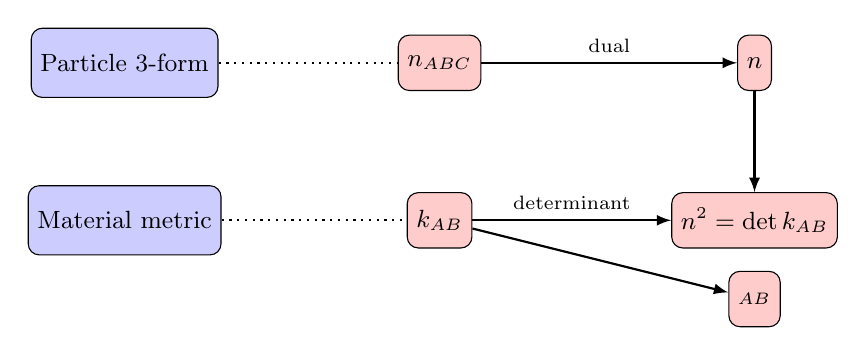
\begin{tikzpicture}[node distance = 2cm, auto]
    % Place nodes
    \node [block2] (form) {{\small Particle 3-form}};
    \node [block, right of=form, node distance=4cm] (form_1) {\small $n_{ABC}$};   
    \node [block, right of=form_1, node distance=4cm] (form_2) {\small $n$};        
    \node [block2, below of=form] (metric) {{\small Material metric}};        
    \node [block, right of=metric, node distance=4cm] (metric_1) {\small $k_{AB}$};     
    \draw [line1] (metric) -- (metric_1);
    \node [block, right of=metric_1, node distance=4cm] (metric_2) {\small $n^2 = \det k_{AB}$};        
    \node [block, below of=metric_2, node distance=1cm] (metric_3) {\small $\unimod_{AB}$};            
    % Draw edges
    \draw [line1] (form) -- (form_1);
    \draw [line] (form_1) -- node{\scriptsize dual}(form_2);
        \draw [line] (metric_1) -- node{\scriptsize determinant}(metric_2);
    \draw [line] (form_2) -- (metric_2);    
       \draw [line] (metric_1) -- (metric_3);        
\end{tikzpicture}
\caption{Explanation of the link between geometrical objects in  the particle 3-form and material-metric formulations of elasticity theory. In the ``particle 3-form'' formulation, the only peice of information about the geometrical structure of the material manifold that is actually used is $n$, the dual of the particle 3-form. In the ``material metric'' formulation, one posits a metric on the material manifold which has more pieces of information which are used: its determinant, $n$, and quantites $\eta_{AB}$ which keep track of the shear-like parts of $k_{AB}$. The point is that the material metric construction keeps track of more information about the material manifold than the particle 3-form construction. In this way the former is more general than the latter.}\label{fig:obj_links}
\end{centering}
\end{figure}
  

The pull-back of the material metric $k_{AB}$ gives a space-time tensor,
\bea
\label{eq:sec:k_abdefn}
k_{ab} = \psi^{\star}k_{AB},
\eea
and will play an important role in what follows.  Specifically, using (\ref{eq:sec:coord-pull-bacj}) the pull-back (\ref{eq:sec:k_abdefn}) reads
\bea
\label{pullbackk}
k_{ab} =  {\psi^A}_a{\psi^B}_b k_{AB}.
\eea
The corrorlary  of   (\ref{eq:sec:ortho-condition}) which we keep coming back to is that   $k_{ab}$ is an orthogonal  space-time field
\bea
u^ak_{ab}=0.
\eea
We will frequently use the  (space-time) tensor with mixed indices; to concrete our notation, space-time indices are raised with the space-time metric,
\bea
\label{eq:sec:defn-kmixed-0}
{k^a}_b = g^{ac}k_{bc}.
\eea
This mixed space-time tensor is also orthogonal,
\bea
\label{eq:sec:orthn-k}
u^a{k^b}_a=0.
\eea
A consequence of (\ref{eq:sec:orthn-k}) is that the indices on $k_{ab}$ can be raised and lowered using the orthogonal space-time metric,
\bea
\label{eq:sec:defn-kmixed}
{k^a}_b = \gamma^{ac}k_{bc}.
\eea
From (\ref{eq:sec:defn-kmixed}) it follows that
\bea
\pd{{k^a}_b}{g^{cd}} = {\delta^a}_{(c}k_{d)b}.
\eea
In a similar fashion,  the pull-back of $\eta_{AB}$ gives an orthogonal space-time tensor
\bea
\label{eq:sec:eta_abdefn}
\eta_{ab} = \psi^{\star}\eta_{AB},
\eea
and we also use the mixed version of the tensor,
\bea
\label{eq:sec:etamixed-defn}
{\eta^a}_b = \gamma^{ac}\eta_{cb}.
\eea
From the pull-back of the relationship (\ref{eq:k-eta-n-defn}) we obtain 
\bea
\label{eq:sec:k-eta-n-pb}
{k^a}_b = n^{2/3}{\eta^a}_b.
\eea

Since we have set everything up so that $n^2$ is the determinant of $k_{ab}$, it follows from (\ref{eq:sec:k-eta-n-pb}) that ${\eta^a}_b$ is a uni-modular tensor:
\bea
\det({\eta^a}_b)=1.
\eea 
This property will be useful later on.

We now elucidate some consequences of the $n$-dependence of $k_{AB}$.
In what follows it will be convenient to denote differentiation with respect to $n$ with a prime. Using (\ref{eq:k-eta-n-defn}) to compute $k_{AB}'$ yields
\bea
\label{eq:sec:tobetraced01}
n\eta'_{AB} = - \tfrac{2}{3}\eta_{AB} + \tau_{AB},
\eea
in which
\bea
\label{defn_tauAB}
\tau_{AB} \defn n^{1/3}k'_{AB}.
\eea
Since $n'_{ABC}=0$ (by definition) it follows that $(\det k_{AB})'=0$, and therefore $k^{-1AB}k_{AB}'=0$, and hence
\bea
\eta^{-1AB}\tau_{AB}=0.
\eea
Thus, we see that $\tau_{AB}$ is   traceless; it is called the \textit{compressional distortion tensor}, and measures   deformations of the medium that \textit{aren't} due to conformal rescalings of the material metric upon varying the particle density.
Hence, computing the trace of (\ref{eq:sec:tobetraced01}) with respect to $\eta^{-1AB}$ yields
\bea
n\eta^{-1AB}\eta'_{AB}=-2.
\eea
Note that from (\ref{defn_tauAB}) it follows trivially, but more usefully, $k'_{AB} = n^{-1/3}\tau_{AB}$, and so if the material varies only  conformally (i.e. is uniformly compressed) $k_{AB}$ is independent of $n$ since $\tau_{AB}=0$ for these types of deformations.


The push-forward of (\ref{eq:sec:tobetraced01}) reads
\bea
n\eta_{ab}' = - \tfrac{2}{3}\eta_{ab} + \tau_{ab}.
\eea
And so, in the case where $\eta_{ab} = \eta_{ab}(n)$, it is simple to see that
\bea
[{\eta}_{ab}]^{\cdot} = \eta'_{ab}[n]^{\cdot},
\eea
where $[X]^{\cdot}$ denotes the material derivative of $X$. After using (\ref{ev_n}) to replace $[n]^{\cdot}=\dot{n}$ we obtain the evolution equation:
\bea
[{\eta}_{ab}]^{\cdot} =  \left( \tfrac{2}{3}\eta_{ab} - \tau_{ab}\right)\Theta.
\eea



\subsection{Material covariant derivative}
It is convenient at this point to introduce the covariant derivative on the material manifold which is compatible with the material metric. Let $\overline{\widetilde{\nabla}}_A$ be the Levi-Civita connection for $k_{AB}$; i.e.,
\bea
\overline{\widetilde{\nabla}}_C k_{AB}=0.
\eea
There is a reason for our including two different ``accents'' above the del-symbol.
The pushed-forward version of $\overline{\widetilde{\nabla}}_A$, denoted as $\overline{\widetilde{\nabla}}_a$, is allowed to act on space-time tensors; note that it will be orthogonal, and so is taken to be the orthogonal projection of some space-time derivative $\widetilde{\nabla}_a$ according to
\bea
\overline{\widetilde{\nabla}}_a{A^{b\cdots}}_{c\cdots} = {\gamma^{d}}_a{\gamma^b}_e\cdots {\gamma^f}_c\cdots\widetilde{\nabla}_d{A^{c\cdots}}_{f\cdots}.
\eea
For any space-time vector $Y^a$ the difference between any two connections can be written as
\bea
\label{eq:sec:intro-d-defn-flsdhfkdgh}
\left(\overline{\widetilde{\nabla}}_a- \overline{\nabla}_a\right)Y^c = {\mathfrak{D}^c}_{ab}Y^b
\eea
in which  $ {\mathfrak{D}^c}_{ab}$ is the (symmetric) relativistic   difference tensor \footnote{The conditions required for this definition to hold are} defined as
\bea
\label{eq:sec:defn-D-ela-diff-tensor}
{\mathfrak{D}^c}_{ab} = \tfrac{1}{2}k^{-1cd}\left( \overline{\nabla}_ak_{bd} + \overline{\nabla}_bk_{ad} - \overline{\nabla}_dk_{ab}\right),
\eea
where $k^{-1cd}$ is defined via
\bea
k^{-1cd} k_{ca} = {\gamma^d}_a, 
\eea
and is orthogonal $ k^{-1cd}u_c = 0$. Due to the applications in mind, we actually call ${\mathfrak{D}^c}_{ab}$ the relativistic elasticity difference tensor.

Using this construction, one finds that $\overline{\widetilde{\nabla}}_a$ is the connection which is compatible with $k_{ab}$,
\bea
\label{bartildenabk=0}
\overline{\widetilde{\nabla}}_ak_{cd} =0.
\eea
As an example of using this technology, suppose that ${B^{a\cdots}}_{b \cdots}$ is a tensor function of $g^{ab}$ and $k_{ab}$. Then taking its derivative with $\overline{\widetilde{\nabla}}_a$  yields
\bea
\overline{\widetilde{\nabla}}_a{B^{b\cdots}}_{c \cdots} = \pd{{B^{b\cdots}}_{c \cdots}}{g^{ef}} \overline{\widetilde{\nabla}}_a{g^{ef}} + \pd{{B^{b\cdots}}_{c \cdots}}{k_{ef}}\overline{\widetilde{\nabla}}_a{k_{ef}}= \pd{{B^{b\cdots}}_{c \cdots}}{g^{ef}} \overline{\widetilde{\nabla}}_a{g^{ef}} ,
\eea
where the second equality holds via (\ref{bartildenabk=0}). We can go one step further and realise that
\bea
\overline{\widetilde{\nabla}}_a{B^{b\cdots}}_{c \cdots} = \pd{{B^{b\cdots}}_{c \cdots}}{g^{ef}} \left(\overline{\widetilde{\nabla}}_a{g^{ef}} -\overline{ {\nabla}}_a{g^{ef}} \right) = 2  \pd{{B^{b\cdots}}_{c \cdots}}{g^{ef}} {\mathfrak{D}^{ef}}_a.
\eea
The second term in braces, $\overline{ {\nabla}}_a{g^{ef}}$, vanishes by (\ref{eq:sec:overlinenabh=0}), and the final equality holds by (\ref{eq:sec:intro-d-defn-flsdhfkdgh}). Finally, since
\bea
\overline{{\nabla}}_a{B^{b\cdots}}_{c \cdots} = \overline{\widetilde{\nabla}}_a{B^{b\cdots}}_{c \cdots}  - \left(  \overline{\widetilde{\nabla}}_a-\overline{{\nabla}}_a\right){B^{b\cdots}}_{c \cdots},
\eea
 then it follows by repeated application of (\ref{eq:sec:intro-d-defn-flsdhfkdgh}) on the last term, that orthogonally projected derivative is
\bea
\label{overlineDB}
\overline{{\nabla}}_a{B^{b\cdots}}_{c \cdots} &=& 2 \pd{{B^{b\cdots}}_{c \cdots} }{g^{de}}{\mathfrak{D}^{de}}_a  - {B^{d\cdots}}_{c\cdots} {\mathfrak{D}^{b}}_{ad} - \cdots + {B^{b\cdots}}_{d\cdots} {\mathfrak{D}^{d}}_{ac} + \cdots. 
\eea




\section{Quantifying the state of the material}
Armed with the map and material metric it remains to understand how to quantify the state of the material. This will guided by understanding the effects of the material on space-time, and is acheived by constructing a material action which can be appended to the Einstein-Hilbert action,  from which one can derive the energy-momentum tensor which sources the gravitational field equations. 

Along the way there are various useful auxiliary quantities, and useful pieces of technology that can be used to help understand what is going on.

 
 
Before we continue it is worth noting some useful ways to compute derivatives of functions which depend on quantities which regularly appear in the construction, most notably functions which depend on $n$ or ${\eta^a}_b$.
First of all, the derivative of the number density $n$ with respect to the space-time metric is given by
\bea
\label{eq:sec:dndg}
\pd{n}{g^{ab}} = \half n \gamma_{ab}.
\eea
When $Y = Y({k^a}_b)$ is any quantity that depends only on the ${k^a}_b$,  then its derivative with respect to the space-time metric is
\bea
\label{eq:pd-Y-g-k}
\pd{Y}{g^{ab}} = k_{c(a}\pd{Y}{{k^{b)}}_c}.
\eea
For any quantity $Z = Z(n,{\eta^a}_b)$, and using (\ref{eq:sec:k-eta-n-pb}) as a decomposition of the degrees of freedom in ${k^a}_b$, we obtain
\bea
\label{eq:sec:Zneta}
\pd{Z}{g^{ab}} = \half n\gamma_{ab}\pd{Z}{n} + \eta_{c\langle a}\pd{Z}{{\eta^{b\rangle}}_c},
\eea
where the angular brackets denote the symmetric trace-free part of the tensor, as defined in (\ref{ttls-defin}). For each quantity $n$, $Y$, and $Z$ as defined here,
\bea
u^a\pd{n}{g^{ab}} =0,\qquad u^a\pd{Y}{g^{ab}}=0,\qquad u^a\pd{Z}{g^{ab}}=0.
\eea
% 
%\note{Fill this in...}
%\bse
%\bea
%\pd{[\rbm{k}]}{g^{ab}} = 
%\eea
%\bea
%\pd{[\rbm{k}^2]}{g^{ab}} = 
%\eea
%\bea
%\pd{[\rbm{k}^3]}{g^{ab}} = 
%\eea
%\ese

\subsection{Constant volume shear tensor}
We define the \textit{constant  volume shear tensor}
\bea
\label{eq:sec:cons-vol-shear-tenor}
{s^a}_b = \tfrac{1}{2}\left( {\gamma^a}_b-{\eta^a}_b \right).
\eea
This is a space-time tensor which quantifies the difference between the actual value of ${\gamma^a}_b$ and the unsheared value ${\eta^a}_b$ as described in Section \ref{sec:mat-metric}. The definition (\ref{eq:sec:cons-vol-shear-tenor}) follows from the pull-back of (\ref{material-space-s}), which was defined in the material manifold.

\note{Do something to build intuition of $s_{ab}$}
\subsection{The equation of state and material action}
\label{sec:eos-introd}
The idea is to quantify the state of the material  from a ``master function'' (to use Carter's terminology). This master function will be the piece of freedom which corresponds to the specification of the type or class of materials under consideration. This is much like the specification of the potential function $V(\phi)$ which controls what types of canonical scalar field theories one is studying. 

For a material, the energy density, $\rho$,    plays the role of the master function; in what follows we will refer to $\rho$ as the \textit{equation of state}. On a first pass  we write down a material action given by the integral of the equation of state which has, as its sole arguments, the mixed components of the pulled-back material metric:
\bea
\label{material-action-k-no-invaraints-1}
\qsubrm{S}{M} =  \int \dd^4x\,\sqrt{-g}\, \rho\left( {k^a}_b\right).
\eea 
This is as far as one can go in generality without asking anything further of the material. 

It is convenient to re-express the equation of state in terms of the particle number density $n$ and the energy per particle, $\epsilon$, via
\bea
\label{eq:decomp_n_rho_ep}
\rho = n\epsilon.
\eea
And so, rather than ask for the form of $\rho$, we ask for the form of $\epsilon$.

\subsection{Variation of the material action and measure-weighted variation}
\label{sec:var-mat-action-mes-we-var}
The material action gives everything we need. But to continue we need to understand how it behaves under application of the variational principle.

Varying the action (\ref{eq:matter-action-material}) yields
\bea
\label{eq;deltaS-material-Diamond-intro}
\delta S = \int \dd^4x\,\sqrt{-g}\, \Diamond\rho.
\eea
We have used the ``diamond derivative'' notation to denote measure-weighted variations, defined to act on a quantity $Q$ via
\bea
\Diamond Q \defn \frac{1}{\sqrt{-g}} \lp\left(\sqrt{-g} Q\right),
\eea
in which $\lp$ is the \textit{Lagrangian variation} operator. The first measure-weighted variation of this quantity $Q$ is
\bea
\label{eq:sec:diamond-Q-first}
\Diamond Q = \lp Q - \tfrac{1}{2}Qg_{ab}\lp g^{ab}.
\eea
The role of $\lp$ is to encorporate both intrinsic variations of a field, and variations due to some other process (such as symmetry transformations). We will return to the explicit description of this operator later on.
Before we  evaluate (\ref{eq;deltaS-material-Diamond-intro}) we want to explain some interesting properties and uses for the first measure-weighted variation.

Let us suppose that $Q$ is a function which depends on a set of scalars $\chi^A$,   their space-time derivatives $\partial_a\chi^A$, and the metric $g_{ab}$,
\bea
Q = Q(\chi^A, \partial_a\chi^A, g_{ab}).
\eea
Then, using (\ref{eq:sec:diamond-Q-first}), we find a rather compact form of the measure-weighted variation of the quantity $Q$:
\bea
\label{eq:diamond-Q-E-T-vatheta]}
\Diamond Q = \mathcal{E}_A\lp \chi^A +\tfrac{1}{2} T_{ab}\lp g^{ab} + \nabla_a\left({\vartheta^a}_A\lp \chi^A\right).
\eea
We have not removed any total derivative terms, and we defined
\bse
\bea
\label{eq:eom_scalars-hkjdfhdkj73982-1-33}
\mathcal{E}_A \defn   \pd{Q}{\chi^A} - \nabla_a\pd{Q}{\partial_a\chi^A},
\eea
\bea
T_{ab} \defn  2\pd{Q}{g^{ab}}  - Qg_{ab} ,
\eea
\bea
{\vartheta^a}_A\defn \pd{Q}{\partial_a\chi^A}.
\eea
\ese
The $\vartheta^a$-term in (\ref{eq:diamond-Q-E-T-vatheta]}) only contributes to the boundary and can be made to vanish by choice of boundary conditions: it won't play a role in what follows. Interpretations of the quantities $\mathcal{E}_A$ and $T_{ab}$ are probably rather obvious, but we will wait for a moment before making concrete statements about what each means.

Now, suppose the variations $\lp$ have two origins: the first is due to diffeomorphisms generated by the vector $\xi^a$, and the second is intrinsic arbitrary variations (of the type usually considered when using variational principles). Then the variations $\lp$ in (\ref{eq:diamond-Q-E-T-vatheta]}) should be replaced with
\bse
\label{lp-ep-lied-lieds}
\bea
\lp = \ep + \lied{\xi},
\eea
in which the  Lie derivatives of the scalars and metric are
\bea
\label{lp-ep-lied-lieds-1}
\lied{\xi} \chi^A =\xi^a\nabla_a\chi^A,\qquad \lied{\xi} g^{ab} = - 2\nabla^{(a}\xi^{b)}.
\eea
\ese
Hence, putting (\ref{lp-ep-lied-lieds}) into (\ref{eq:diamond-Q-E-T-vatheta]}) yields
\bea
\label{eq:diamondQ-fhdfjgdkhfd-field-gen}
\Diamond Q =\mathcal{E}_A\ep \chi^A +\tfrac{1}{2} T_{ab}\ep g^{ab}+ \xi^a\left( \mathcal{E}_A \nabla_a\chi^A+ \nabla^{b}T_{ab}  \right)- \nabla_{a}S^a  ,
\eea
in which
\bea
S^a \defn  \xi^{b}\left({T^a}_b - {\vartheta^a}_A\nabla_b\chi^A\right) - {\vartheta^a}_A\ep \chi^A.
\eea
The final term only contributes to the boundary, and vanishes identically in the absence of the scalars in the scenario where $\xi^{a}T_{ab}=0$. This could be the case, for example, if $\xi^a \propto u^a$  and $T_{ab} \propto \gamma_{ab}$ only. We can read off from (\ref{eq:diamondQ-fhdfjgdkhfd-field-gen}) that diffeomorphism invariance is ensured when the coefficient of the diffeomorphism generating field $\xi^a$ vanishes, namely when
\bea
\label{eq:eom_scalars-hkjdfhdkj73982-1}
\nabla^{b}T_{ab}=-\mathcal{E}_A \nabla_a\chi^A.
\eea
We can also read off from (\ref{eq:diamondQ-fhdfjgdkhfd-field-gen}) that the condition for the theory to be stationary under arbitrary variations in the scalars $\chi^A$ is that the coefficient  of the arbitrary variations $\ep \chi^A$ should vanish, i.e.,
\bea
\label{eq:eom_scalars-hkjdfhdkj73982}
\mathcal{E}_A =0.
\eea
It is immediately clear from its definition (\ref{eq:eom_scalars-hkjdfhdkj73982-1-33}) that the conditions (\ref{eq:eom_scalars-hkjdfhdkj73982}) are just the Euler-Lagrange equations of motion of the scalars $\chi^A$. By inspecting (\ref{eq:eom_scalars-hkjdfhdkj73982-1}) it is manifest   that  the satisfaction of theequations of motion (\ref{eq:eom_scalars-hkjdfhdkj73982}) implies conservation of the energy-momentum tensor. 

Let us now return to the   problem at hand: evaluation of (\ref{eq;deltaS-material-Diamond-intro}) for the material medium. At the top of Section \ref{sec:eos-introd} we stated that the equation of state $\rho$ (i.e. the integrand of the material action) is a function of the pulled-back metric ${k^a}_b$ alone, (\ref{material-action-k-no-invaraints-1}). This means that $\lp\rho$ can be written as
\bea
\label{eq:sec:vary-rho-1}
\lp\rho = \pd{\rho}{g^{ab}}\lp g^{ab},
\eea
which can be used to obtain
\bea
\label{eq:eom_scalars-hkjdfhdkj73982-4637}
\Diamond\rho = \half \left( - \rho g_{ab} + 2\pd{\rho}{g^{ab}}\right)\lp g^{ab}.
\eea
We remind that (\ref{eq:eom_scalars-hkjdfhdkj73982-4637}) is the integrand of the first variation of the action. 

\subsection{The energy-momentum tensor}
We have in mind that the material constitutes only part of the dynamics of the entire ``universe'': there is also the  possibility of gravitational dynamics (not nessecarily limited to those prescribed by General Relativity), and also other matter,  fluid, or scalar-field sources. In the case that General Relativity provides the gravitational dynamics, the gravitational field equations are given by
\bea
G_{ab} = 8 \pi G \sum_{\rm i} \qsuprm{T}{i}_{ab},
\eea
where $\qsuprm{T}{i}_{ab}$ is the energy-momentum tensor for the $\qsuprm{\rm i}{th}$ source. Below we will be concerned with computing the energy-momentum tensor for the material. We will only use the symbol $T_{ab}$ for the material's energy-momentum tensor, but one should keep in mind that it can be added to any additional energy-momentum tensors.

The energy-momentum tensor is   derived from varying the material action $\qsubrm{S}{M}$ using the usual expression,
\bea
\label{emt-defn-variation}
T_{ab} = - \frac{2}{\sqrt{-g}}\frac{\delta \qsubrm{S}{M}}{\delta g^{ab}}.
\eea
The quantity in braces in (\ref{eq:eom_scalars-hkjdfhdkj73982-4637}) is precisely the variation requires to work out the right-hand-side of (\ref{emt-defn-variation}); and so, the energy-momentum tensor is given by 
\bea
\label{eq:sec:TAB_material-pre-ortho}
T_{ab} = - \rho g_{ab} + 2\pd{\rho}{g^{ab}}.
\eea
We are able to further evaluate this expression, and in particular we can deduce   the ``types'' of contributions to $T_{ab}$ from knowledge of what $\rho$ is a function of. Since the equation of state only depends on the mixed components of the pulled-back material metric,
\bea
\label{eq:eos-assumed-form}
\rho = \rho\left({k^a}_b\right),
\eea
using (\ref{eq:pd-Y-g-k}) gives an expression for the final term in (\ref{emt-defn-variation}):
\bea
\pd{\rho}{g^{ab}} = k_{c(a}\pd{\rho}{{k^{b)}}_c}.
\eea
Since the right-hand-side of this expression is orthogonal by virtue of (\ref{eq:sec:orthn-k}), so is the left-hand-side,
\bea
\label{eq:eom_scalars-hkjdfhdkj73982-4637-1}
u^a\pd{\rho}{g^{ab}} =0.
\eea
And so, assuming an equation of state $\rho$ has been given in the form of (\ref{eq:eos-assumed-form}), the energy-momentum tensor of the solid (\ref{eq:sec:TAB_material-pre-ortho}) can be written as
\bse
\bea
\label{eq:sec:emt-solid}
T_{ab} = \rho u_au_b + P_{ab},
\eea
in which the pressure tensor $P_{ab}$ is given by
\bea
\label{pressuretensor}
P_{ab} = 2 \pd{\rho}{g^{ab}} - \rho \gamma_{ab}.
\eea
\ese
By virtue of (\ref{eq:eom_scalars-hkjdfhdkj73982-4637-1}) the pressure tensor (\ref{pressuretensor}) is orthogonal,
\bea
 u^aP_{ab}=0.
\eea
The important thing to note is that there is no heat flux term in $T_{ab}$:
\bea
u^a{\gamma^b}_c T_{ab} = 0.
\eea
This a consequence of the orthogonality of the mapping between the material manifold and spacetime. 

After using the solid form of the energy-momentum tensor (\ref{eq:sec:emt-solid}), the variation of the energy density (\ref{eq:sec:vary-rho-1}) can be written as
\bea
\lp\rho = \tfrac{1}{2}\left( \rho \gamma_{ab} + P_{ab}\right)\lp g^{ab}.
\eea


After rewriting the equation of state $\rho$ in terms of an energy per particle, $\epsilon$, via (\ref{eq:decomp_n_rho_ep}),  the pressure tensor (\ref{pressuretensor}) takes on  the more compact form
\bea
\label{eq:sec:pab-eps}
P_{ab} = 2n\pd{\epsilon}{g^{ab}}.
\eea
When the energy per particle $\epsilon$ is written in a (still general) way to only depend on the number density $n$ and the components of the  uni-modular tensor ${\eta^a}_b$, i.e., 
\bea
\epsilon = \epsilon(n, {\eta^a}_b),
\eea
we can use (\ref{eq:sec:Zneta}) to further evaluate the pressure tensor (\ref{eq:sec:pab-eps}), yielding the rather attractive expression
\bea
\label{eq:sec:press-scal-aniso}
P_{ab} = p \gamma_{ab} + \pi_{ab} ,
\eea
in which  we have identified the pressure scalar $p$,
\bse
\bea
\label{iso-ess}
p = n^2\pd{\epsilon}{n},
\eea
and the (traceless) anisotropic stress tensor
\bea
\label{anso-press}
\pi_{ab} = 2 n \eta_{c\langle a}\pd{\epsilon}{{\eta^{b\rangle}}_c}.
\eea
We remind that the energy density is given by
\bea
\rho = n \epsilon.
\eea
\ese
This highlights that dependence of $\epsilon$ on the number density $n$ is linked to isotropic pressure $p$, and dependence of $\epsilon$ on the uni-modular tensor ${\eta^a}_b$ is linked to anisotropic stress $\pi_{ab}$. Note that $n$ is the determinant of the material metric, and ${\eta^a}_b$ encodes the ``other'' invariants.

There is nothing ``imperfect'' about the construction of the substance so far: there is no dissipation,   everything is conserved, and is constructed from a very geometrical point of view. However, the pressure tensor (\ref{eq:sec:press-scal-aniso}) has anisotropic stress (\ref{anso-press}). For a \textit{fluid} this would signal an imperfection, but it is exactly this anisotropic stress which makes the theory  that of a  \textit{solid}.

It has recently become popular to suggest that an observation of anisotropic stress would point towards modified gravity rather than dark energy \cite{Bellini:2014fua, Saltas:2014dha, Amendola:2014wma, Linder:2014fna}. What we are about to state is not a comment on a claim made by any of these articles, but it is worth pointing out. Whilst it is true that modified gravity models have anisotropic stress, it is also true that material models can contribute towards anisotropic stress. Infact, material models constitute the simplest and physically ``most intuitive'' additions to the Einstin-Hilbert and standard matter content gravitational model.



\section{Equation of motion and propagation of sound}
Obtaining the equation of state and energy-momentum tensor is clearly only part of the story. One must also obtain equations of motion: these come from the conservation equation
\bea
\label{eq:sec:cons-eq-gen}
\nabla_aT^{ab}=0.
\eea
If the material is the only source to the gravitational field equations, then (\ref{eq:sec:cons-eq-gen}) follows by diffeomorphism invariance, and also by the Bianchi identity. If there are multiple sources to the gravitational field equations, then (\ref{eq:sec:cons-eq-gen}) holds if and only if $T^{ab}$ is interpreted as the sum of the individual energy-momentum tensors (of which the material's EMT can be an additive contribution). Only in  the case when these sources are ``decoupled'', their individual energy-momentum tensors are independently conserved.

We will proceed by first proving this statement, then continue by providing a useful way to write down  (\ref{eq:sec:cons-eq-gen}) in a rather physically intuitive manner.

\subsection{Equations of motion from the action}
Without assuming the existence of the pulled-back material metric, one should be convinced that the action will be a function of the metric $g^{ab}$,  a set of scalars $\phi^A$ representing the particle positions in the material manifold, and their derivatives $  \partial_a\phi^A$. There may  be other material space tensors, but we shall leave that complicating possibility out for now. With these considerations, the action can be written as
\bea
\qsubrm{S}{M} = \int \dd^4x\,\sqrt{-g}\, \rho\left( g^{ab}, \phi^A, \partial_a\phi^A\right).
\eea
Under Lagrangian variations $\lp$ in the available fields, $g^{ab}$ and $\phi^A$, the corresponding  measure-weighted variation of the action density  is
\bea
\label{material-diamondrho-fgdfkj-1}
\Diamond\rho =  \tfrac{1}{2} T_{ab} \lp g^{ab} - \mathcal{E}_A\lp \phi^A .
\eea
Recall that measure-weighted variation was  discussed  in section \ref{sec:var-mat-action-mes-we-var}.
We set $T_{ab}$ to be the energy-momentum tensor, as defined in the usual manner, 
\bea
T_{ab} = - \frac{2}{\sqrt{-g}}\frac{\delta \qsubrm{S}{M}}{\delta g^{ab}} = 2\pd{\rho}{g^{ab}} - \rho g_{ab},
\eea
and the contribution  multiplying the perturbed scalars is
\bea
\mathcal{E}_A = \nabla_a\left( \pd{\rho}{\partial_a{\phi^A}}\right)- \pd{\rho}{\phi^A} .
\eea

The symbol $\lp$     stands for the  arbitrary variation operator which acts on the fields which we defined in (\ref{lp-ep-lied-lieds}). For the metric $g^{ab}$ and the set of scalars $\phi^A$   the relevant expressions for the Lie derivative is given by (\ref{lp-ep-lied-lieds-1}). 
After integrating by parts and neglecting the total derivative, the measure-weighted  variation in the action density (\ref{material-diamondrho-fgdfkj-1}) becomes
\bea
\label{eq:diff-var-SM}
\Diamond\rho = \tfrac{1}{2}T_{ab} \ep g^{ab} - \mathcal{E}_A\ep \phi^A + \xi^a \left( \nabla^bT_{ab} - \mathcal{E}_A\nabla_a\phi^A\right).
\eea

This can be used to obtain the functional derivative of the action with respect to the intrinsic variations in the scalars,
\bea
\label{eq:eom_EA}
\frac{\Diamond\rho }{\ep \phi^A} = - \mathcal{E}_A.
\eea
The variational principle demands that this expression must vanish, and yields the equation of motion satisfied by the scalars $\phi^A$.
General covariance requires the action to be invariant under changes in the coordinates. We read off from (\ref{eq:diff-var-SM}) that an arbitrary coordinate transformation  can be performed and not affect the material action when the coefficient of $\xi^a$ vanishes:
\bea
\label{eq:sec:cons_eom}
\nabla^bT_{ab} = \mathcal{E}_A\,\partial_a\phi^A.
\eea
This links  conservation of energy-momentum and the equations of motion of the scalars. Put another way: energy-momentum conservation implies the satisfaction of the equations of motion of the elastic medium. At first glance it seems that the system is overdetermined: there are three scalars $\phi^A$ which are supposed to have equations of motion, but there are four components to (\ref{eq:sec:cons_eom}). This apparent over-determination is resolved by the orthogonality of the map.

The orthogonality of the mapping (\ref{eq:sec:ortho-condition})    can be written as
\bea
u^a\partial_a\phi^A = 0,
\eea
and so therefore the time-like projection of (\ref{eq:sec:cons_eom}) is automatically satisfied:
\bea
u^a\nabla^bT_{ab}=0.
\eea
It then follows that the orthogonal projection of (\ref{eq:sec:cons_eom}) implies the vanishing of (\ref{eq:eom_EA}):
\bea
{\gamma^a}_c\nabla^bT_{ab} =0\qquad \Longleftrightarrow\qquad \mathcal{E}_A=0.
\eea
Therefore, conservation of energy-momentum guarantees that the scalars $\phi^A$ satisfy their equation of motion.

\subsection{The fluid equations}
Inspired by the result of the previous section, we now present the conservation equations in a physically intuitive manner. One must constantly keep in mind that satisfaction of the equations of motion is equivalent to energy-momentum conservation.

Using the solid form (\ref{eq:sec:emt-solid}) for $T_{ab}$ the two independent (i.e., time-like and orthogonal) projections of the conservation equation (\ref{eq:sec:cons-eq-gen}) are
\bse
\bea
\label{eq:sec:density-cons}
\dot{\rho} + (\rho \gamma^{ab} + p^{ab})\Theta_{ab}=0,
\eea
\bea
\label{eq:sec:pressure-cons}
(\rho \gamma^{ab} + p^{ab})\dot{u}_b + \overline{\nabla}_bp^{ab}=0.
\eea
\ese
We used the orthogonally projected derivative $\overline{\nabla}_b$, as defined in (\ref{eq:orth-proj-deri-defn})

If the energy per particle $\epsilon$ is a function only of the components ${k^a}_b$, then using (\ref{eq:sec:pab-eps}) in conjunction with (\ref{overlineDB}), the orthogonally projected derivative of the pressure tensor can be written as
\bea
\label{eq:sec:overlineP}
\overline{\nabla}_bp^{ab} = \left({E^{ab}}_{cd} - {\gamma^{a}}_c{p^b}_d\right){\mathfrak{D}^{cd}}_b,
\eea
in which we used the elasticity difference tensor ${\mathfrak{D}^{cd}}_b$ as defined in (\ref{eq:sec:defn-D-ela-diff-tensor}), and introduced     the relativistic \textit{elasticity tensor},  ${E^{ab}}_{cd}$, defined via
\bea
\label{eq:defn-E-1}
{E^{ab}}_{cd} \defn 2\pd{p^{ab}}{\gamma^{cd}} - p^{ab}\gamma_{cd}.
\eea  
It is manifest from this definition that the elasticity tensor has the following symmetries in its indices:
\bea
\label{eq:defn-E-12}
E^{abcd} = E^{(ab)(cd)}.
\eea
Using (\ref{eq:sec:dndg}) and (\ref{eq:sec:pab-eps}),   the elasticity tensor can be written  as the second derivative of the energy per particle $\epsilon$ via
\bea
\label{eq:defn-E-2}
E^{abcd} = 4n \pd{^2\epsilon}{\gamma_{ab}\partial \gamma_{cd}}.
\eea
This final relationship informs us that the elasticity tensor is also symmetric under interchange of the first and last pair of indices, 
\bea
\label{eq:defn-E-2222}
E^{abcd} = E^{cdab}
\eea
in addition to the simple symmetries (\ref{eq:defn-E-12}).

It will be convenient to use the relativistic \textit{Hadamard elasticity tensor},  ${A^{ab}}_{cd}$, defined via the elasticity tensor via
\bea
\label{eq:defn-rel-hadamard-1}
{A^{ab}}_{cd} \defn {E^{ab}}_{cd} - {\gamma^{a}}_c{p^b}_d.
\eea
Using the Hadamard elasticity tensor, the orthogonally projected derivative of the pressure tensor (\ref{eq:sec:overlineP}) takes on a particularly simple form,
\bea
\overline{\nabla}_bp^{ab} ={A^{ab}}_{cd}{\mathfrak{D}^{cd}}_b,
\eea
and the orthogonal projection (\ref{eq:sec:pressure-cons}) of the conservation equations can be written as
\bea
(\rho \gamma^{ab} + p^{ab})\dot{u}_b +A^{abcd}\mathfrak{D}_{cbd}=0.
\eea


A rather convenient form of the equations of motion is given in \cite{Carter21111972, Carter:1973zz}; in terms of the material derivative \note{need to explain the material derivative somewhere} the pressure tensor satisfies
\bea
\left[p^{ab}\right]^{\cdot} = - p^{ab}\theta - E^{abcd} \theta_{cd}.
\eea
In the more usual notation of ``time-like'' derivatives, the equations of motion for the materials energy density and pressure tensor are given by
\bse
\bea
\label{eq:sec:time-cons-shfkds-prof}
u^a\rho_{;a}= - \rho {u^a}_{;a} - p^{ab}u_{a;b},
\eea
\bea
\label{eq:sec:time-cons-shfkds-prof-b}
u^c{p^{ab}}_{;c} = 2 p^{c(a}{u^{b)}}_{;c} + 2 p^{c(a}u^{b)}\dot{u}_c - p^{ab}{u^c}_{;c}  - E^{abcd}u_{c;d},
\eea
\ese
where we defined  the acceleration vector $\dot{u}_a = u^b\theta_{ab}$. Specification of the components of the elasticity tensor, which must be subject to the symmetries (\ref{eq:defn-E-12}) and (\ref{eq:defn-E-2222}), closes the fluid equations.
\subsection{Speed of sound}
The story so far has led to us being able to write down the equations of motion, with all freedom being contained within the components of the elasticity tensor. We will now perform a calculation with these equations, and setup the equations into a particular physical configuration which will enable us to  compute the speed of sound of the medium \cite{Carter:1973zz}. This calculation requires the introduction of many quantities: they are collected with brief definitions in Table \ref{tab:common-soundspeed}.

Sound wavefronts are characteristic hypersurfaces across which the acceleration vector $\dot{u}^a$ has a jump discontinuity (the velocity $u^a$ and the metric remain continuous). Following Carter, we denote discontinuities across the wavefront with square braces; and so we set
\bea
\label{eq:sec:dot-u-disc}
\left[\dot{u}^a\right] = \alpha \iota^a,
\eea 
in which $\alpha$ is the amplitude of the wavefront and $\iota^a$ is the polarization vector satisfying the space-like normalization condition, $\iota^a\iota_a=1$.
Since the acceleration and velocity vectors are mutually orthogonal, $u_a\dot{u}^a=0$,
it follows that the polarization vector and the velocity vector are orthogonal $u_a\iota^a=0$.
The \textit{propagation direction vector} $\nu^a$ is specified with the same orthonormality conditions as the polarization vector, namely $\nu^a\nu_a = 1$ and $\nu^au_a=0$.


{\renewcommand{\arraystretch}{1.4}
\begin{table}%[b] 
%\begin{andptabular}{X[4c]X[4c] }%
\begin{center}
\begin{tabular}{||c |  L ||}
%{Summary  of    commonly used symbols}
\hline
\textbf{Symbol} & \textbf{Meaning} \\
\hline
$[X]$ & Discontinuity of $X$ across the sound wave-front\\\hline
$\alpha$ & Amplitude of acceleration discontinuity\\\hline
$\iota^a$ & Space-like polarization vector\\\hline
$\nu^a$ & Propagation direction vector\\\hline
$\lambda_a = \nu_a - v u_a$ & Normal of the wave-front\\\hline
$v = u^a\lambda_a$ & Sound speed\\ \hline
$\{\sigma, \kappa^a, \tau^{ab}\}$ & Amplitude of discontinuity of the derivative of \{density, velocity, pressure tensor\} on wave-front
\\\hline
\end{tabular}\caption{Summary of the  symbols used to compute the sound speed}\label{tab:common-soundspeed}
\end{center}
\end{table}
}

The normal to the characteristic hypersurface is in the direction of the vector $\lambda_a$, defined via
\bea
\lambda_a = \nu_a - vu_a.
\eea
The scalar 
\bea
v = \lambda^au_a
\eea
is the speed of propagation.

The derivatives of the density, velocity, and pressure tensor fields on the characteristic hypersurface are given in terms of quantities $\sigma, \kappa^a, \tau^{ab}$ via
\bse
\label{sos_hfdhfkd_abc}
\bea
\label{sos_hfdhfkd_a}
\left[ \rho_{;a}\right] = \sigma \lambda_a,
\eea
\bea
\label{sos_hfdhfkd_b}
\left[ {u^a}_{;b}\right] = \kappa^a\lambda_b,
\eea
\bea
\left[ {p^{ab}}_{;c}\right] = \tau^{ab}\lambda_c.
\eea
\ese
We now show how to determine the values of $\sigma, \kappa^a, \tau^{ab}$ in terms of $v, \alpha$, and $\iota^a$. First, contracting (\ref{sos_hfdhfkd_b}) with $u^b$ gives (\ref{eq:sec:dot-u-disc}) on the left-hand-side, and $v\kappa^a$ on the right-hand-side, and thus one obtains
\bse
\label{eq:sec:found-stuff-dhskjdk-1}
\bea
v\kappa^a = \alpha \iota^a.
\eea
Taking the discontinuity of the   projections of the conservation equation (\ref{eq:sec:time-cons-shfkds-prof}) and (\ref{eq:sec:time-cons-shfkds-prof-b}), and then multiplying by $v$ respectively yields
\bea
v^2\sigma = - \alpha \left( \rho \iota^a\lambda_a + p^{ab}\iota_a\lambda_b \right),
\eea
\bea
v^2\tau^{ab} = \alpha\left( 2vu^{(a}p^{b)c}\iota_c + 2p^{c(a}\iota^{b)}\lambda_c - p^{ab}\iota^c\lambda_c - E^{abcd}\iota_c\lambda_d \right).
\eea
\ese

Putting the general form of the energy-momentum tensor (\ref{eq:sec:emt-solid}) into the conservation equation (\ref{eq:sec:cons-eq-gen})
\bea
\label{eq:sec:gen_disc}
\left( u^b\rho_{;b} + \rho{u^b}_{;b} \right)u^a + \rho \dot{u}^a + {p^{ab}}_{;b}=0.
\eea
Taking the discontinuity of the general formula (\ref{eq:sec:gen_disc}) and using (\ref{sos_hfdhfkd_abc}) yields
\bea
\left( v\sigma + \rho \kappa^b\lambda_b\right)u^a + \rho \alpha \iota^a + \tau^{ab}\lambda_b=0.
\eea
Now using (\ref{eq:sec:found-stuff-dhskjdk-1}) for $\kappa^a, \sigma$, and $\tau^{ab}$ yields
\bea
\label{character-1}
v^2\left( \rho \gamma^{ab} + p^{ab}\right)\iota_b + p^{bc}\lambda_b\lambda_c\iota^a - E^{abcd}\lambda_b\iota_c\lambda_d=0.
\eea
By using the relativistic Hadamard tensor $A^{abcd}$, defined in (\ref{eq:defn-rel-hadamard-1}),  the equation (\ref{character-1}) becomes
\bea
\label{eq:sec:characteriztif-khgdj-1}
\left[v^2\left( \rho \gamma^{ab} + p^{ab}\right)  - Q^{ab}\right]\iota_b=0.
\eea
where we have introduced the Fresnel tensor $Q^{ab}$ which is defined in terms of the Hadamard tensor and the propagation vector $\nu_a$ via
\bea
Q^{ac} \defn A^{abcd}\nu_b \nu_d,
\eea
after noting that the Hadamard tensor is orthogonal on all indices. Orthogonality of the Hadamard tensor carries over to give orthogonality of the Fresnel tensor,
\bea
u_aQ^{ab}=0.
\eea
Since every term in the characterstic equation (\ref{eq:sec:characteriztif-khgdj-1}) is orthogonal, it is essentially a 3-dimensional  equation. The eigenvalues $v^2$ are the squared sound speed (in general there will be three values).


Although we will show where this comes from later on, it is worth our providing an example of the explicit computation of the sound speed. In the case of an isoptropic elastic solid close to a ground state, the pressure tensor is specified in terms of the isotropic pressure scalar as $p^{ab} = p \gamma^{ab}$, and the elasticity tensor is given by
\bea
\label{eq:sec:per-solid-e-kfdkfh-ss}
E^{abcd} = \left( \beta - \tfrac{1}{3}p\right)\gamma^{ab}\gamma^{cd} + 2 \left( \mu + p\right) \left( \gamma^{a(c}\gamma^{d)b} - \tfrac{1}{3}\gamma^{ab}\gamma^{cd}\right);
\eea
the coefficients $p, \beta$, and $\mu$, are repectively the isotopic pressure, bulk modulus, and  modulus of rigidity. The Hadamard tensor in this case is given by
\bea
A^{abcd} = \beta \gamma^{ab}\gamma^{cd} + 2 p\gamma^{a[d}\gamma^{b]c} + 2 \mu\left( \gamma^{a(c}\gamma^{d)b} - \tfrac{1}{3}\gamma^{ab}\gamma^{cd}\right),
\eea
and the Fresnel tensor works out as
\bea
Q^{ab} = \left( \beta + \tfrac{1}{3}\mu\right) \nu^a\nu^b + \mu \gamma^{ab}.
\eea
Hence, the characteristic equation (\ref{eq:sec:characteriztif-khgdj-1}) becomes
\bea
\left[ v^2\left(\rho + p \right) \gamma^{ab} - \mu \gamma^{ab} - \left( \beta + \tfrac{1}{3}\mu\right)\nu^a\nu^b \right]\iota_b=0.
\eea
There are two solutions: the first is where the polarization   and propagation vectors are aligned, $\nu_a = \iota_a$ in which case the eigenvalue is
\bea
v^2 = \frac{\beta + \tfrac{4}{3}\mu}{\rho+p}\defn \qsubrm{c}{L}^2.
\eea
Secondly, where the polarization and propagation vectors are orthogonal: $\nu_a\iota^a=0$, in which case the eigenvalue is
\bea
v^2 = \frac{\mu}{\rho+p}\defn \qsubrm{c}{T}^2.
\eea
We therefore have two sound speeds; $\qsubrm{c}{L}^2$ which is the speed of propagation of longitudinal modes, and $\qsubrm{c}{T}^2$ which is the speed of propagation of transverse modes.
 

\section{The isotropic solid}
So far we have not asked anything of the solid. We can however ask (or, demand, depending on your point of view) that the solid is isotropic. That is, invariant under $SO(3)$ transformations of the material coordinates. What this ends up imposing is that the action is dependent only upon scalar invariants formed from the pulled-back material metric. In this section we show what these invariants are,  the resulting action, and give an example equation of state.
\subsection{Constructing scalar invariants}
\label{sec-setscalinvs}
We are interested in constructing the allowed arguments of the equation of state $\rho$.  When the material is constrained to be isotropic, the arguments of this equation of state are formed from  scalar invariants of the available material tensors. From the point of view of the theoretical construction which concerns us at the moment, this requires an understanding of the allowed scalar quantities one can form from objects which specify the state of the system.  The scalar invariants are constructed from the pull-back of the material metric, ${k^a}_b$.

There are a few different sets of scalar invariants one could use: formally they will be identical, but different choices will help or hide  insight  into the  physical behavior. There are two, ultimately equivalent, sets of scalar invariants which we now describe.

As a candidate set of invariants,   \textit{the} three independent scalar invariants of the mixed components of the pulled-back material metric ${k^a}_b$ are
\bea
\label{invs-i1i2i3}
I_1 = [\rbm{k}],\qquad I_2 = [\rbm{k}^2],\qquad I_3 = [\rbm{k}^3],
\eea
in which we   denoted   traces with square braces,
\bea
I_n = \Tr(\rbm{k}^n) = [\rbm{k}^n] = {k^a}_b{k^b}_c\cdots{k^f}_a ,
\eea
with ${k^a}_b$ defined from $k_{ab}$ via (\ref{eq:sec:defn-kmixed}). To reiterate, (\ref{invs-i1i2i3}) is a complete list of independent invariants due to the orthogonality of ${k^a}_b$ (\ref{eq:sec:orthn-k}), and any other invariants can be computed from these via the Cayley-Hamilton theorem. For example, since $n_{ABC}$ is the volume form of $k_{AB}$, the particle number density $n$ is also a scalar invariant of ${k^a}_b$; by the Cayley-Hamilton theorem, the determinant is related to the other invariants via
\bea
n^2 = \det({k^a}_b) = \tfrac{1}{3!}\left([\rbm{k}]^3 - 3[\rbm{k}][\rbm{k}^2] + 2 [\rbm{k}^3]\right).
\eea

We  could use $\{I_1,I_2,I_3\}$ as defined in (\ref{invs-i1i2i3}) as the list of invariants for the arguments of the equation of state, but we shall also consider the particle number density $n$ and  the independent scalar invariants of the uni-modular tensor ${\eta^a}_b$, defined in (\ref{eq:sec:etamixed-defn}) since this will help the comparison between solid and fluid descriptions. The important consequence of   uni-modularity is that     ${\eta^a}_b$   only has two independent invariants (rather than 3 which could be expected from a symmetric rank-2 tensor in 3D).  The invariants are linked via the Cayley-Hamilton theorem as
\bea
\label{eq:sec:eta-link-invariants}
3! = [\gbm{\eta}]^3 - 3 [\gbm{\eta}][\gbm{\eta}^2] + 2 [\gbm{\eta}^3].
\eea

And so, in brief summary, we have  shown that there are two  equivalent   ways to write the most general function of state for a solid with scalar arguments: both have a maximum of three arguments. They are
\bse
\bea
\rho = \rho\left([\rbm{k}],\left[\rbm{k}^2\right],\left[\rbm{k}^3\right]\right)
\eea 
and
\bea
\label{eos-scal-n-eta}
\rho = \rho\left(n, [\gbm{\eta}],\left[\gbm{\eta}^2\right]\right).
\eea
\ese
We remind that ${k^a}_b$ is the pull-back of a tensor whose volume form is $n_{ABC}$ and (squared) determinant is the particle number density, $n$, and that  ${\eta^a}_b$ is a uni-modular tensor whose inverse $\eta^{-1AB}$ co-incides with the push-forward of the space-time metric when the material is in the unsheared state. The latter formulation, (\ref{eos-scal-n-eta}), is somewhat favorable, since it becomes easy to connect to a scenario in which the solid ``becomes'' like a fluid, since $\rho$ becomes independent of the $[\gbm{\eta}^n]$.
\subsection{The action of an isotropic solid}
When one demands that the material is isotropic then this constitutes a constraint on  $\rho$ as being a  function of any possible scalar invariants discussed in Section \ref{sec-setscalinvs}. With this constraint imposed, the material action is given the integral of a tri-variate scalar function,
\bea
\label{eq:matter-action-material}
\qsubrm{S}{M} = \int \dd^4x\,\sqrt{-g}\, \rho\left([\rbm{k}],\left[\rbm{k}^2\right],\left[\rbm{k}^3\right]\right).
\eea
And so, rather than ask for the form of $\rho$, we ask for the form of $\epsilon$, and then write the matter action (\ref{eq:matter-action-material}) as
\bea
\qsubrm{S}{M} = \int \dd^4x\,\sqrt{-g}\, n \epsilon\left([\rbm{k}],\left[\rbm{k}^2\right],\left[\rbm{k}^3\right]\right).
\eea
\subsection{Example equation of state}
It is instructive to specify an example equation of state and obtain the energy-momentum tensor. We will make the same choice as described in \cite{Karlovini:2002fc}, and write down a particular equation of state (which is only a subset of all the possible models) for isotropic materials.    

To begin with it is useful to recall the covariant form of the constant volume shear tensor (\ref{eq:sec:cons-vol-shear-tenor}), which we repeat here for completeness:
\bea
s_{ab} = \tfrac{1}{2}(\gamma_{ab} - \eta_{ab}).
\eea
There are two methods to raise indices (and thus construct traces). These methods are
\bea
{s^a}_b = \gamma^{ac}s_{cb},\qquad {\hat{s}^a}{}_b = \eta^{-1ac}s_{cb}.
\eea
In matrix form these respectively read
\bea
\rbm{s} = \tfrac{1}{2}(\rbm{1} - \gbm{\eta}),\qquad \hat{\rbm{s}} = \tfrac{1}{2}(\gbm{\eta}^{-1} - \rbm{1}).
\eea
The equation of state  $\epsilon$ is chosen  to be a function of the particle number density $n$ and a particular combination of the invariant of ${\eta^a}_b$. The explicit form of $\epsilon$ is
\bea
\label{eq:sec:epsilon-pick-form-example}
\epsilon = \check{\epsilon}_0(n) + \frac{\check{\mu}(n)}{n}\overline{s}^2,
\eea
in which $\overline{s}^2$ is the shear scalar defined from the invariants of ${\eta^a}_b$ via
\bea
\label{eq:sec:s2-choice-1}
\overline{s}^2 \defn \tfrac{1}{36}\left( [\gbm{\eta}]^3 -[\gbm{\eta}^3] - 24\right).
\eea
Notice that by using the Cayley-Hamilton relation (\ref{eq:sec:eta-link-invariants}), the choice of shear scalar (\ref{eq:sec:s2-choice-1}) is equivalent to
\bea
\overline{s}^2 = \tfrac{1}{24}\left( [\gbm{\eta}]^2 - [\gbm{\eta}^2] \right)[\gbm{\eta}] - \tfrac{3}{4}.
\eea
Using (\ref{eq:sec:epsilon-pick-form-example}) the material action is therefore given by
\bea
\qsubrm{S}{M} = \int \dd^4x\,\sqrt{-g}\,  \bigg\{ n\check{\epsilon}_0 +  \tfrac{1}{36}{\check{\mu}}{ }\left( [\gbm{\eta}]^3 -[\gbm{\eta}^3] - 24\right)\bigg\}.
\eea
The pressure tensor is given by (\ref{eq:sec:press-scal-aniso}) where the isotropic pressure scalar (\ref{iso-ess}) is  
\bse
\bea
\label{example_isotp-jfghdkhfgdj}
p = \check{p} + (\check{\Omega}-1)\sigma,
\eea
and the anisotropic stress (\ref{anso-press}) is given by
\bea
\pi_{ab} = \tfrac{1}{6}\check{\mu}\left([\gbm{\eta}]^2 \eta_{\langle ab\rangle} - \eta^{cd}\eta_{c\langle a}\eta_{b\rangle d} \right),
\eea
\ese
and where the three quantities appearing in the pressure (\ref{example_isotp-jfghdkhfgdj}) are
\bea
 \check{p} = n^2\frac{\dd \check{\epsilon}_0}{\dd n},\qquad \check{\Omega} = \frac{n}{\check{\mu}}\frac{\dd\check{\mu}}{\dd n},\qquad\sigma = \check{\mu}s^2.
\eea




\section{The Carter-Quintana perfect solid}
Carter and Quintana conclude their paper with an exposition of the equations for a \textit{perfect elastic solid}.  Before we give their equation of state and energy-momentum tensor, we shall discuss physical issues regarding the existence (or otherwise) of locally relaxed states of the material. See also \cite{Lukacs:1976ja} for a presentation of  FRW solutions to the Carter-Quintana elastic solid system.
\subsection{Strain and shear tensors}
The strain tensor is linked to the assumption about the existence of a locally relaxed state of a material -- this is the unstrained state. In the unstrained state the energy per particle $\epsilon$ is supposed to be minimum when $\gamma_{ab}$ takes on a particular value, $k_{ab}$ say. This invites a quantification of the state of strain of the material by measuring the difference between the actual value of $\gamma_{ab}$ and its unstrained value $k_{ab}$ via the \textit{strain tensor}, $e_{ab}$, defined as
\bea
e_{ab} = \tfrac{1}{2}\left( \gamma_{ab} - k_{ab}\right).
\eea
Recalling that the energy per particle is denoted as $\epsilon$, we define $\epsilon_0$ to be the energy per particle in the unstrained state. The Hookean idealization takes the energy per particle to be of quadratic form in the strain tensor
\bea
\epsilon = \epsilon_0 + \tfrac{1}{2}K^{abcd}e_{ab}e_{cd}.
\eea
The elasticity tensor $E^{abcd}$ relates to $K^{abcd}$ via
\bea
E^{abcd} = n K^{abcd}.
\eea
Hence, since $\rho = n \epsilon$, the energy density can be written as
\bea
\rho = \frac{n}{n_0}\rho_0 + \tfrac{1}{2}E^{abcd}e_{ab}e_{cd},
\eea
and the pressure tensor is related to the strain tensor via
\bea
p^{ab} = - E^{abcd}e_{cd}.
\eea
The tensor $k_{ab}$ can be thought of as a Riemannian metric on material space; the pull-back formalism means that $u^ak_{ab}=0$. 
Associated with the  value $\epsilon_0$ of $\epsilon$  in the unstrained state are the values $\rho_0$ of the energy density $\rho$, and $n_0$ of the particle number density $n$.
 
The complication which Carter invites is that not all physical systems of interest will have a state which is locally relaxed, thus negating the existence of $k_{ab}$ and rendering this construction impotent. This leads to the introduction of the shear tensor.

Rather than ask for the relaxed state to be a state where the energy per particle is minimum, we ask for a state in which $\epsilon$ is minimized subject to the restriction of constant particle number density. This is the unsheared state, and motivates the introduction of $\eta_{ab}(n)$ which is the value of $\gamma_{ab}$ in the unsheared state with particle number density $n$. Again, to quantify the state of shear we define the \textit{constant volume shear tensor} via
\bea
s_{ab} = \tfrac{1}{2}\left( \gamma_{ab} - \eta_{ab}\right),
\eea
which (to reinforce the point) is the difference between the actual value of $\gamma_{ab}$ and its value in the unsheared state.

We define $\check{\rho}(n)$ to be the energy density in the unsheared state, and hence
\bea
\check{\rho} = n \check{\epsilon}.
\eea
When $\epsilon$ does have an absolute minimum, at some particle number density $n_0$, one can keep the previous notions of the strain tensor; indeed
\bse
\bea
\eta_{ab}(n_0) &=& k_{ab},\\
\check{\rho}(n_0) &=& \rho_0,\\
\check{\epsilon}(n_0) &=& \epsilon_0.
\eea
\ese

\subsection{The equation of state}
The ``physics'' of the solid that Carter and Quintana had in mind was that it was supposed to have vanishing compressional distortion. That is, the compressional distortion tensor is supposed to vanish, $\tau_{ab}=0$. This means that  the reference tensors satisfy
\bse
\bea
[\eta_{ab}]^{\cdot} = \tfrac{2}{3}\eta_{ab}\Theta,
\eea
\bea
[\eta^{-1ab}]^{\cdot} = - \tfrac{2}{3}\eta^{-1ab}\Theta,
\eea
and the strain tensor satisfies
\bea
[s_{ab}]^{\cdot} = \tfrac{2}{3}s_{ab}\Theta + \sigma_{ab}.
\eea
\ese
Here, $[X]^{\cdot}$ denotes the \textit{material derivative} of $X$ (this is explained the first half of Carter and Quintana, and we will do so later on).
One can obtain
\bea
\eta_{ab} = (n/n_0)^{-2/3}k_{ab},
\eea


The solid is supposed to be isotropic with respect to its unsheared states. Hence, the energy per particle (recall, $\rho = \epsilon n$, and $\epsilon$ is the energy per particle) is a function only of invariants. There are a maximum of three invariants: they are taken to be the particle number density $n$ and the two independent invariants of the shear tensor ${s^a}_b$. The particular combination of these are taken to be
\bse
\bea
s^2 \defn \left( \eta^{-1ad}\eta^{-1bc} - \tfrac{1}{3}\eta^{-1ab}\eta^{-1cd}\right)s_{ab}s_{cd}=  \lceil\rbm{s}^2\rceil - \tfrac{1}{3}\lceil\rbm{s}\rceil^2,
\eea
\bea
l \defn\eta^{-1ab}\eta^{-1cd}\eta^{-1ef}s_{bc}s_{de}s_{fa}= \lceil\rbm{s}^3\rceil.
\eea
\ese
We used the   notation $\lceil\rbm{X}\rceil$ for traces which are taken with $\eta^{-1ab}$ (as opposed to $[\rbm{X}]$ which was used to denote traces with $g^{ab}$): this choice is for simplicity of the resulting formulae and does not lose generality.  Recall  that the shear tensor $s_{ab}$ is related to the material metric $k_{ab}$ and particle number density via
\bea
k_{ab} = n^{2/3}\left( \gamma_{ab} - 2 s_{ab}\right).
\eea

Hence, the most general form of the equation of state is a function with three arguments:
\bea
\epsilon = F(n,s^2,l).
\eea
The action for Einsteinian gravity with the CQ  solid is thus
\bea
S = \int \dd^4x\,\sqrt{-g}\, \left[ \frac{R}{16\pi G} - n F(n,s^2,l)\right].
\eea
\subsection{The energy-momentum tensor}
The energy density $\rho$,  and pressure tensor $p^{ab}$ are given by
\bse
\bea
\label{CQPF-rho}
\rho = nF,
\eea
\bea
\label{CQPF-press-tens}
p^{ab} &=& \left\{n^2F_{,n} + ns^2\left( \frac{4}{3}F_{,s^2} + F_{,l}\right) - n \left( 2l+ \tfrac{1}{3}\lceil\rbm{s}\rceil^2\right)F_{,l} \right\}\gamma^{ab}\nonumber\\
&& - 2n F_{,s^2}\left(\eta^{-1a(c}\eta^{-1d)b} - \tfrac{1}{3}\eta^{-1ab}\eta^{-1cd} \right)s_{cd}\nonumber\\
&& - 3nF_{,l}\eta^{-1a(c}\eta^{-2d)b}\eta^{-1ef}s_{ce}s_{df}.
\eea
\ese
These expressions contain the corrections to the typos which were present in \cite{Carter21111972}, and which were pointed out (by the same authors) in \cite{Carter:1977qf}. The isotropic pressure is found from the trace of (\ref{CQPF-press-tens}), and is given by
\bea
\label{CQPF:eq:press-scal}
p = n^2F_{,n} + 2n\left( \frac{2}{3}s^2F_{,s^2}- l F_{,l}\right).
\eea


\subsection{Slow roll parameter}
We take this opportunity to recall that for inflating an FLRW Universe one requires smallness of the slow-roll parameter $\qsubrm{\epsilon}{slow}$, defined as
\bea
\label{slow-roll-defn}
\qsubrm{\epsilon}{slow} \defn - \frac{\dot{H}}{H^2} = \frac{3(\rho+P)}{2\rho}.
\eea
Using (\ref{CQPF-rho}) and (\ref{CQPF:eq:press-scal}) the slow-roll parameter (\ref{slow-roll-defn}) evaluates for the CQ perfect solid to give
\bea
\label{eq:sec:sr-eval-1}
\qsubrm{\epsilon}{slow} = \frac{3}{2}\left[ 1+\pd{\log F}{\log n}+ \frac{4}{3}\pd{\log F}{\log s^2} - 2\pd{\log F}{\log l} \right].
\eea
The structure of (\ref{eq:sec:sr-eval-1}) suggests a separable ansatz for the functional form of $F$:
\bea
F(n,s^2,l) = x(n)y(s^2)z(l),
\eea
since (\ref{eq:sec:sr-eval-1}) becomes
\bea
\qsubrm{\epsilon}{slow} = \frac{3}{2}\left[ 1 + nx' + \frac{4}{3}s^2y' - 2 lz'\right],
\eea
in which a prime is used to denote derivative with respect to the sole argument of the given function.

\section{The solid action}
Recall from (\ref{eq:matter-action-material}) that the action for the solid can be written as a tri-variant function whose arguments are the three independent scalar invariants formed from the mixed-components of the pulled-back material metric:
\bea
S = \int \dd^4x\, \sqrt{-g}\, \ld\left( [\rbm{k}], [\rbm{k}^2], [\rbm{k}^3]\right).
\eea
Our focus in this section is on providing useful ways to construct workable sub-theories from this action.

\subsection{Derivative counting}
Suppose we counted the terms by keeping track of the number of derivatives. The pulled-back material metric ${k^a}_b$ has two space-time derivatives, and so the $\qsubrm{n}{th}$-trace has $2n$-inverse-powers of a mass-scale $M$,
\bea
[\rbm{k}^n] \sim \frac{1}{M^{2n}}.
\eea
We can use this to write the complete list of terms in the solid-action which come with a given power of $M$. Up to sixth-order the Lagrangian density is 
\bea
\ld =\frac{1}{M^2} b\,[\rbm{k}] + \frac{1}{M^4} \left(c_1\, [\rbm{k}^2] + c_2\, [\rbm{k}]^2\right) + \frac{1}{M^6}\left(d_1\,[\rbm{k}^3] + d_2\,[\rbm{k}][\rbm{k}^2] + d_3\,[\rbm{k}]^3 \right) + \ldots.
\eea
We have introduced the dimensionless coefficients, $\{b, c_i, d_i\}$, to control the strength which which a given term influences the action.

\subsection{The quasi-Hookean solid}
We will make use of the notation 
\bse
\bea
\check{\epsilon}(n) &=& F(n,0,0),\\
\check{\rho}(n) &=& nF(n,0,0),\\
\check{p}(n) &=& n^2\pd{F}{n}(n,0,0),\\
\beta(n) &=& n^3\pd{^2F}{n^2}(n,0,0) + 2n^2\pd{F}{n}(n,0,0),\\
\mu(n) &=& n\pd{F}{s^2}(n,0,0).
\eea
\ese
The quantities $\check{\rho}, \check{p}, \beta, \mu$ are the unsheared energy density, bulk  and rigidity moduli.
The value of the elasticity tensor in the state of zero shear strain is
\bea
\check{E}^{abcd}(n) = (\beta - \tfrac{1}{3}\check{p})\eta^{-1ab}\eta^{-1cd} + 2(\mu + \check{p})( \eta^{-1a(c}\eta^{-1b)d} - \tfrac{1}{3}\eta^{-1ab}\eta^{-1cd}).
\eea
Note that this is the elasticity tensor we computed the sound speeds for just after equation (\ref{eq:sec:per-solid-e-kfdkfh-ss}).


The Lagrangian for the Carter-Quintana solid in the  quasi-Hookean limit (which we shall refer to as a ``quasi-Hookean solid'') is linear in $s^2$, and independent of $l$:
\bea
\qsubrm{F}{qHs} = \check{\epsilon} + \tfrac{\mu(n)}{n}s^2.
\eea
For this quasi-Hookean solid the energy density and pressure tensor are respectively given by
\bse
\bea
\rho = \check{\rho} + \mu s^2,
\eea
\bea
p^{ab} = \left\{ \check{p} + \left( n\mu' + \tfrac{1}{3}\mu\right)s^2 \right\}\gamma^{ab} - 2 \mu\left\{  \eta^{-1a(c}\eta^{-1b)d} - \tfrac{1}{3}\eta^{-1ab}\eta^{-1cd}\right\}s_{cd}.
\eea
\ese

\subsection{Solid $\rightarrow$ fluid $\rightarrow$ $\Lambda$}
The theory, as constructed, is the general description for a perfect solid. The particular solid under examination is determined by the dependance of $\epsilon$ on its   arguments. This is simple to impose,   has interesting consequences, and  the physics alters in a meaningful way.  For example, when
\bea
\epsilon\left(n, {\eta^a}_b\right) \longrightarrow \epsilon(n),
\eea
  the anisotropic stress tensor (\ref{anso-press}) vanishes, and one is left with a theory which describes a perfect fluid. Furthermore, when 
\bea
\epsilon(n) = \frac{\epsilon_0}{n},
\eea
where $\epsilon_0$ is a constant, one finds that $\rho = - p$.  That is, the theory is that of a cosmological constant (the Lagrangian is just $\ld = \epsilon_0$, a constant).
\section{Perturbed solids}
The majority of this review has been focussed on the general theory of solids: the deformations performed on the solid or medium may be arbitrarily large. Whilst this is very general, it also yields a theory which is complicated to work with. There are a substantial number of physical systems for whom the non-linear theory of elasticity is ``over-kill'': understanding the governing equations that describe small deformations of the solid from its equilibrium configuration is often sufficient. For this reason we shall review the theory of perturbed solids.

Comprehensive reviews, applications, and examples in the relativistic theory have already been presented \cite{Carter:1973zz, Carter:1977qf, Bucher:1998mh, Battye:2005ik, Battye:2007aa, Battye:2013er, Pearson:2014iaa}, as well as the non-relativistic theory being the main subject of a classic book by Landau and Lifshitz \cite{ll_elast}.

The physical picture one should constantly keep in mind is that a continuous medium has ``two states'': relaxed and deformed. The former occurs when there are no forces on the medium, and the latter will induce strains and forces on other surrounding materials and fields (notably the metric). In some sense the ``point'' of a model is to catalogue the possible ways in which a material can influence surrounding media and fields. 



\subsection{Non-relativistic solids}
A non-relativistic solid is one for whom there are no gravitational effects. As examples, one imagines an eraser, rubber band, trampolines: these kinds of materials. Another distinguishing feature of non-relativistic solids from relativistic ones is that the pressure of the solid is negligible.

The locations within a relaxed non-relativistic solid are denoted by $x^i$. Under a deformation the coordinates alter according to 
\bea
x^i \longrightarrow x^i + \xi^i(x^j).
\eea
 If the line element in the solid before the deformation is $\dd\ell^2 = \delta_{ij} \dd x^i \dd x^j$, then after the deformation the line element has metric  given by
\bea
g_{ij} = \delta_{ij} + 2 \varepsilon_{ij},
\eea
in which we defined the strain tensor,
\bea
\label{non-rel-strain-defn}
\varepsilon_{ij}\defn \partial_{(i}\xi_{j)}.
\eea
The components of the strain tensor $\varepsilon_{ij}$ contain all information about the deformation performed on the body. We now require information about the manner in which the body responds to the given deformation. This   entails   an understanding of the stress tensor, $\sigma^{ij}$, for a given strain tensor $\varepsilon_{ij}$. This is where the ``physics'' comes in.

Although this seems like a tangential calculation, consider that if one computes the divergence of the stress tensor one obtains the components of the force. These can be equated to the acceleration of the deformation vectors to obtain the equation of motion
\bea
\label{nonrela-eom}
F^i = \partial_j\sigma^{ij} = \rho \ddot{\xi}^i.
\eea
And so, if the stress tensor can be related to the strain tensor (which, we remind is constructed from the derivatives of the deformation vector), then the equation of motion (\ref{nonrela-eom}) becomes a closed set of equations.

In broad-brush-terms there are two cases which are useful to consider and describe a huge class of physically useful solids.
\begin{enumerate}
\item The stress tensor is proportional to the strain tensor:
\bea
\label{e-solid}
\sigma^{ij} = E^{ijkl}\varepsilon_{kl}.
\eea
The components,   $E^{ijkl}$, precisely prescribe the strength of certain forces for given deformations (we will have much more to say about this later); they are the components of the elasticity tensor, and there are a fixed number of them for any given material in a space-time with given dimension. This ``given number'' is rather large for a material with arbitrary symmetry, but dramatically reduces once the material is imposed to have certain symmetries. Materials for whom (\ref{e-solid}) holds are   Hookean elastic solids.
\item The stress tensor is proportional to the rate-of-strain tensor:
\bea
\label{v-solid}
\sigma^{ij} = V^{ijkl}\dot{\varepsilon}_{kl}.
\eea
The components   $V^{ijkl}$ play a similar role to the components of the elasticity tensor for a Hookean solid, except here we are  considering viscous solids and $V^{ijkl}$ are the components of the viscosity tensor.
\end{enumerate}
Of course, the given physical material may require an amalgamation of the two cases, whereby stress is proportional to both strain, and rate-of-strain, in which case
\bea
\label{kv-solid}
\sigma^{ij} = E^{ijkl}\varepsilon_{kl}+ V^{ijkl}\dot{\varepsilon}_{kl}.
\eea
The expression (\ref{kv-solid}) describes visco-elastic solids (also known as Kelvin-Voigt solids). Since (\ref{kv-solid}) contains both the elastic (\ref{e-solid}) and viscous (\ref{v-solid}) models as sub-cases, we will proceed with the Kelvin-Voigt expression (\ref{kv-solid}). Using (\ref{non-rel-strain-defn}) and (\ref{kv-solid}), the equation of motion (\ref{nonrela-eom}) is
\bea
\label{eom-kv-nonreal}
\rho \ddot{\xi}^i = E^{ijkl}\partial_j\partial_{(k}\xi_{l)} + V^{ijkl}\partial_j\partial_{(k}\dot{\xi}_{l)}. 
\eea

The problem of describing the solid considerably simplifies when one assumes some symmetry of the solid, for example material isotropy. In such cases (other symmetries require more freedom than we are about to introduce), the material tensors only have two independant components each, and decompose completely as
\bse
\label{decomp_iso}
\bea
E^{ijkl} = \left(\beta-\tfrac{2}{3}\mu\right) g^{ij}g^{kl} + 2\mu g^{i(k}g^{l)j},\\
V^{ijkl} = \left(\lambda-\tfrac{2}{3}\nu\right) g^{ij}g^{kl} + 2\nu g^{i(k}g^{l)j}.
\eea
\ese
Using the decompositions (\ref{decomp_iso}), the stress-tensor (\ref{kv-solid}) becomes
\bea
\sigma^{ij} = \left( \beta - \tfrac{2}{3}\mu\right) g^{ij}\partial_k\xi^k + \left( \lambda - \tfrac{2}{3}\nu\right) g^{ij}\partial_k\dot{\xi}^k + 2\mu \partial^{(i}\xi^{j)} + 2 \nu\partial^{(i}\dot{\xi}^{j)},
\eea
and the equation of motion (\ref{eom-kv-nonreal}) becomes
\bea
\label{iso-eom}
\rho \ddot{\xi}^i = \left( \beta + \tfrac{1}{3}\mu\right) \partial^i\partial_k\xi^k + \mu \partial_k\partial^k\xi^i + \left( \lambda + \tfrac{1}{3}\nu\right) \partial^i\partial_k\dot{\xi}^k + \nu \partial_k\partial^k\dot{\xi}^i.
\eea

We shall provide a simple example which highlights the seperate modes of propagation inherent in a material medium. Consider the simple case where the deformation vector has only two components; we can expand $\xi^i$ using two scalars $\phi$ and $\psi$ in an orthonormal basis $(\hat{x}^i, \hat{y}^i)$ via
\bse
\label{iso-eom-ex}
\bea
\xi^i = \phi\hat{x}^i + \psi\hat{y}^i.
\eea
Now suppose that these scalars depend on time, and only one of the two available spatial directions; that is, we set
\bea
\partial_i\phi = \phi'\hat{x}_i,\qquad \partial_i\psi = \psi'\hat{x}_i.
\eea
\ese
Putting the decomposition of the deformation vector (\ref{iso-eom-ex}) into the equation of motion (\ref{iso-eom}) yields an equation with two independant projections (one along $\hat{x}^i$, and one along $\hat{y}^i$); these projections leads to the requirement that the following two equations are satisfied:
\bea
\ddot{\phi} - \frac{\lambda + \frac{4}{3}\nu}{\rho}\dot{\phi}'' = \frac{\beta+\frac{4}{3}\mu}{\rho}\phi'',\qquad
\ddot{\psi} - \frac{\nu}{\rho}\dot{\psi}'' = \frac{\mu}{\rho}\psi''.
\eea
In the purely elastic case (i.e., where all components of the viscosity tensor vanish), it is with relative ease that one realises a plane wave ansatz $\phi \sim e^{\ci\left( \omega t + kx \right)}$ solves the equations of motion, and that $\phi$ and $\psi$ travel with different speeds: these are the  longitudinal and transverse sound speeds
\bea
\qsubrm{c}{L}^2 = \frac{\beta + \frac{4}{3}\mu}{\rho},\qquad \qsubrm{c}{T}^2 = \frac{\mu}{\rho}.
\eea
\subsection{Relativistic solids}
In the relativistic theory one needs to carefully describe the perturbations; there are intrinsic variations in the metric, and pre-existing matter fields, as well as perturbations in the continuous medium.  

The coordinates of the undeformed medium are represented by $\overline{x}^a$, and those of the deformed medium are by $x^a$. These are related via
\bea
 x^a =  \overline{x}^a+\xi^a(x^b) .
\eea
The crucial piece here is the deformation vector, $\xi^a(x^b)$, which as have we explicitly shown via our notation, is dependent upon the space-time coordinates (different locations can deform by different amounts).

The metric of a space-time which contains a perturbed medium is given by expanding the metric to linear order in intrinsic metric perturbations, $h_{ab}$, and in the deformation vector,
\bea
\label{metric-perts-elastic}
g_{ab} = \overline{g}_{ab} +h_{ab} + 2 \nabla_{(a}\xi_{b)}.
\eea
The metric of the unperturbed space-time is $\overline{g}_{ab}$, and the metric fluctuations due to ``intrinsic'', or extra-material contents, is given by $h_{ab}$. The presence of the perturbed medium is encapsulated by the term involving the deformation field, 
\bea
\xi^a = x^a - \overline{x}^a.
\eea
One may recognise the final term in (\ref{metric-perts-elastic}) as that which arises in standard perturbation theory after one performs the diffeomorphism 
\bea
\label{eq:def-exo-pert-2dgsjd-1}
x^a\rightarrow x^a + \xi^a(x^b).
\eea
Of course, this recognition is accurate. There is an additional concept to appreciate however: interpretation. The $\xi^a$-field describes all the fluctuations of the medium away from its equilibrium configuration. In addition, the deformation field $\xi^a$ is orthogonal,
\bea
\label{eq:def-exo-pert-2dgsjd-1-2}
u_a\xi^a=0.
\eea
The key to obtaining a picture of whats going on here is to go back to the construction we laid out in section \ref{sec:mpnd}, and imagine that the solid in space-time is a collection of particles, each of which traces out its own world-line.  The deformation represented by (\ref{eq:def-exo-pert-2dgsjd-1}), and constrained by (\ref{eq:def-exo-pert-2dgsjd-1-2}), should be interpreted as a given world-line being moved from its original trajectory. Or, to use a more cohesive language: the world-lines are being deformed.
\subsubsection{Lagrangian and Eulerian variations}
A more elegant, and geometrically intuitive way to write the corrections to the metric is by writing all of the non-background terms in (\ref{metric-perts-elastic}) as
\bea
\label{ep-lp-liedx-metric}
\lp g_{ab} = \ep g_{ab} + \lied{\xi}g_{ab},
\eea
in which we identified the intrinsic metric perturbation as
\bea
\ep g_{ab} \defn h_{ab},
\eea
and the usual expression for the Lie derivative of the metric along the vector $\xi^a$,
\bea 
\lied{\xi}g_{ab} = 2\nabla_{(a}\xi_{b)}.
\eea
The expression (\ref{ep-lp-liedx-metric}) encapsulates a more general framework of Lagrangian and Eulerian variations, and how they are related in a system which is deformed.  This distinction is only valid or useful in systems where the metric has intrinsic perturbations, possibly of the type usually considered in, say cosmological perturbatino theory. 
\subsubsection{The perturbed energy-momentum tensor}
The field equations for the perturbations (in the conventional sense) of a gravitating system which only contains an elastic medium are given by
\bea
\ep   G^{\mu\nu} = 8 \pi G\, \ep   T^{\mu\nu},
\eea
where we used the symbol ``$\ep$'' to denote intrinsic variations. The source term, $\ep   T^{\mu\nu}$, is constructed from a term which contains the variations in the energy-momentum tensor 
\bea
\ep T^{\mu\nu} = \lp T^{\mu\nu} -\lied{\xi}T^{\mu\nu}.
\eea
\bea
\lied{\xi}T^{\mu\nu} = \xi^{\alpha}\nabla_{\alpha}T^{\mu\nu} - 2T^{\alpha(\mu}\nabla_{\alpha}\xi^{\nu)}
\eea
In the visco-elastic case,
\bea
\lp T^{\mu\nu} = - \half \left( W^{\mu\nu\alpha\beta}  + T^{\mu\nu} g^{\alpha\beta} \right) \lp g_{\alpha\beta} - V^{\mu\nu\alpha\beta} \lp K_{\alpha\beta};
\eea
\bea
W^{\mu\nu\alpha\beta} = E^{\mu\nu\alpha\beta} + P^{\mu\nu}u^{\alpha}u^{\beta} + P^{\alpha\beta}u^{\mu}u^{\nu} - 4 u^{(\alpha}P^{\beta)(\mu}u^{\nu)} - \rho u^{\mu}u^{\nu}u^{\alpha}u^{\beta}
\eea
The elasticity and viscosity tensors have the symmetries
\bea
E^{\mu\nu\alpha\beta} = E^{(\mu\nu)(\alpha\beta)} = E^{\alpha\beta\mu\nu},\qquad V^{\mu\nu\alpha\beta} = V^{(\mu\nu)(\alpha\beta)} ,
\eea
and are  orthogonal on all indices,
\bea
u_{\mu}E^{\mu\nu\alpha\beta}=0,\qquad u_{\mu}V^{\mu\nu\alpha\beta} = u_{\alpha}V^{\mu\nu\alpha\beta} = 0.
\eea
\subsection{Deformations about a relaxed state}
It is   important to understand how to deal with a deformed medium. Before we give some explicit expressions for  deformations of the solid, we shall illustrate the philosophy via ``non-linear sigma models'' from field theory.
\subsubsection{Example from non-linear sigma models}
One of the important ideas in continuous mechanics is that of the assumed existence of a relaxed state: this is supposed to be some configuration that minimizes some measure of ``energy''. This concept is absolutely vital in the study of solitons. As the simplest example, consider the Lagrangian density for a real scalar field $\phi$ living in a Higgs potential,
\bea
\label{eq:lag-dw-1}
\ld = - \half \partial_{a}\phi\partial^{a}\phi - \frac{\lambda}{4}\left( \phi^2 - \eta^2\right)^2.
\eea
The relaxed configuration of this scalar is when $\phi = \pm \eta$ (commonly known as the vacuum manifold). It is simple to find the Lagrangian density for fluctuations about the relaxed state; substituting $\phi = \eta + \delta\phi$ into (\ref{eq:lag-dw-1}) and expanding to quadratic order in $\delta\phi$ yields
\bea
\ld = - \half \partial_{a}\delta\phi\partial^{a}\delta\phi - \half \lambda \eta^2(\delta\phi)^2.
\eea
The Lagrangian that results is that for a massive scalar field, and it describes the perturbations about the relaxed state. 

This example was simple enough to demonstrate the idea of a ``relaxed state'' in a non-linear field theory, but it was in some sense ``too'' simple since there isn't a non-trivial Lagrangian that describes the field \textit{in} the relaxed state. For that we shall move to a more complicated example and think about a multi-scalar field model whose Lagrangian density is
\bea
\label{eq:sec:lag-full}
\ld =- \half \mathfrak{k}_{IJ}\partial_{a}\Phi^I\partial^{a}\Phi^J- V(\Phi^I).
\eea
There are supposed to be $n$ fields here, and so $I = 1, \ldots, n$, and the set of symmetric quantities $ \mathfrak{k}_{IJ}$ are supposed to play the role of a  metric in field space.
Before we continue we want to make it plainly clear that this isn't the most general Lagrangian density that can be constructed out of single derivatives. 

 Suppose that the energy gets minimized when the fields $\Phi^I$ are consigned to live on a sub-manifold, $\mathcal{V}$ say, of dimension $q \leq n$; in this state the potential energy $V(\Phi^I)=0$. The ``vacuum manifold'' $\mathcal{V}$ can be coordinatized by $q$ scalars $\phi^A$, say, with $A = 1, \ldots, q$. Hence, when the configuration is in its relaxed state the original set of fields $\Phi^I$ are expressible as a function of the fields $\phi^A$,
\bea
\label{eq:sec:relaxed-config}
\Phi^I = \Phi^I(\phi^A).
\eea
By simple application of the chain rule,  (\ref{eq:sec:relaxed-config}) provides
\bea
\label{eq:sec:parti-phiI-phiA}
\partial_{a}\Phi^I = \pd{\Phi^I}{\phi^A}\partial_{a}\phi^A.
\eea
Putting (\ref{eq:sec:parti-phiI-phiA}) into (\ref{eq:sec:lag-full}) gives 
\bea
\label{eq:lag-eff-phiA}
\ld = - \half \mathfrak{g}_{AB}(\phi)\partial_{a}\phi^A\partial^{a}\phi^B,
\eea
in which we defined
\bea
\label{eq:sec:GAB-met}
\mathfrak{g}_{AB}(\phi) \defn  \mathfrak{k}_{IJ}\pd{\Phi^I}{\phi^A}\pd{\Phi^J}{\phi^B}.
\eea
The $\mathfrak{g}_{AB}$ are interpreted as the components of the metric on the field submanifold $\mathcal{V}$.   The field equations for the $\phi^A$ derived from (\ref{eq:lag-eff-phiA})   are given by
\bea
g^{ ab}\nabla_{a}\nabla_{b}\phi^A + \cs{A}{B}{C}\nabla_{a}\phi^B\nabla^{a}\phi^C=0,
\eea
where
\bea
\label{eq:cs-sigmamodel}
\cs{A}{B}{C} = \tfrac{1}{2} \mathfrak{g}^{AD}\left( \partial_B\mathfrak{g}_{CD} + \partial_C\mathfrak{g}_{BD} - \partial_D\mathfrak{g}_{BC} \right)
\eea
are the Christoffel symbols for   the metric in the field submanifold.

One of the simplest ways (we can think of, at least) to see how study fluctuations or deformations  away from the relaxed state  is to first imagine that the relaxed state is specified by the condition
\bea
\label{eq:sec:relxed-cond}
\pd{\Phi_0^I}{\phi_0^A} = {\mathfrak{J}^I}_A ,
\eea
where   the ``0'' subscripts are used to specify that the configuration is relaxed, and the gothic-J is used to denote the relaxed Jacobian. Using (\ref{eq:sec:relxed-cond}) to compute (\ref{eq:sec:GAB-met}) gives a simple expression for the submanifolds metric in the relaxed state,
\bea
\overline{\mathfrak{g}}_{AB} = \mathfrak{k}_{IJ}{\mathfrak{J}^I}_A{\mathfrak{J}^J}_B .
\eea
It should be evident that the Christoffel symbols in the field submanifold (\ref{eq:cs-sigmamodel}) are   zero for this relaxed state if $\mathfrak{k}_{IJ}$ is flat and the Jacobians ${\mathfrak{J}^I}_A={\delta^I}_A$. We have denoted $\overline{\mathfrak{g}}_{AB}$ as the field submanifolds metric in the relaxed state. In a deformed state the derivatives of $\Phi^I$ with respect to the $\phi^A$ must differ from their values in the relaxed state by some amount which can be packaged into a rank-2 tensor ${\mathfrak{d}^I}_A$ (this is a gothic-d, for ``deformation'') via
\bea
\label{eq:strainfksgkfhgfmhgdf-12}
\pd{\Phi^I}{\phi^A} = {\mathfrak{J}^I}_A + {\mathfrak{d}^I}_A,
\eea
where we will not make any assumptions about the size of the ${\mathfrak{d}^I}_A$.  Putting (\ref{eq:strainfksgkfhgfmhgdf-12}) into (\ref{eq:sec:GAB-met}) gives
\bea
\mathfrak{g}_{AB} =\overline{\mathfrak{g}}_{AB} + 2 \mathfrak{d}_{AB} + {\mathfrak{d}^I}_A\mathfrak{d}_{IB}.
\eea
This expression is very similar to what is used in  the non-linear Stuckelberg trick in the massive gravity literature (see, e.g., \cite{Hinterbichler:2011tt, deRham:2014zqa}). It is therefore apparent that the deviation of $\mathfrak{g}_{AB}$ from $\overline{\mathfrak{g}}_{AB}$ is contained within the tensor
\bea
s_{AB} = \mathfrak{d}_{AB} + \tfrac{1}{2}{\mathfrak{d}^I}_A\mathfrak{d}_{IB},
\eea
so that
\bea
s_{AB} = \tfrac{1}{2} \left(\mathfrak{g}_{AB} -\overline{\mathfrak{g}}_{AB} \right).
\eea
Hence, we now have a measure on how deformed the material is: when $s_{AB}=0$ one has $\mathfrak{g}_{AB} = \overline{\mathfrak{g}}_{AB}$ which is the relaxed metric, and any $s_{AB}\neq 0$ means that the material is deformed in some way. If the deformations are small then one can safely assume that $\mathfrak{d}_{AB}$ is a small quantity and so $S_{AB}  = \mathfrak{d}_{AB}$.
\subsubsection{Deformations of the material}
To make more explicit contact to the construction we gave in section \ref{sec:mpnd}, suppose that the actual values of the material coordinates $\phi^A$ are related by way of an ``expansion'' (which is not necessarily small) about some fiducial state whose coordinates were $\overline{\phi}{}^A$. That is,
\bea
\phi^A = \overline{\phi}{}^A + \pi^A.
\eea
Then the configuration gradient (\ref{eq:sec:config_gradient}) can be evaluated 
\bea
\label{eq:configu_deformed}
{\psi^A}_a = {\overline{J}}{}^A{}_a + \partial_a\pi^A,
\eea
in which the configuration gradient computed in the fiducial state is
\bea
{\overline{J}}{}^A{}_a = \pd{\overline{\phi}{}^A }{x^a}.
\eea
Using (\ref{eq:configu_deformed}) to provide an expression for the configuration gradient to compute the pull-back $k_{ab}$ of the material metric $k_{AB}$  via (\ref{pullbackk}) yields
\bea
k_{ab} = \overline{k}_{ab}+2\partial_{(a}\xi_{b)}+ \Pi_{ab},
\eea
in which we defined
\bse
\bea
\overline{k}_{ab}&\defn& k_{AB} {\overline{J}}{}^A{}_a{\overline{J}}{}^B{}_b ,\\
\partial_a\xi_b &\defn& k_{AB}{\overline{J}}{}^A{}_a\partial_b\pi^B ,\\
\Pi_{ab} &\defn& k_{AB} \partial_a\pi^A\partial_b\pi^B. 
\eea
\ese
The $\Pi_{ab}$-term is neglected if the deformations are small. The quantity $\overline{k}_{ab}$ is the pull-back of the material metric when the material is in its unstrained state (i.e. when the $\pi^A=0$ identically). 

It should thus be clear that important information about the state of the system is the contained within the tensor
\bea
S_{ab} \defn \half \left( k_{ab} - \overline{k}_{ab}\right),
\eea
since it quantifies the difference between the actual value of $k_{ab}$ and its value in the fiducial state.


\section{Final remarks}